\chapter{Nucleon Decay and Atmospheric Neutrinos}
\label{ch:physics-atmpdk}

\section{Nucleon Decay}
\label{sec:physics-atmpdk-ndk}

\subsection{Physics Motivation}
%The class of theories known as Grand Unified Theories (GUTs) makes
%predictions about both baryon number violation and proton lifetime
%that may be within reach of the full-scope DUNE experiment.
Grand Unified Theories (GUTs)  unite the three gauge interactions of particle 
physics -- strong, weak, and electromagnetic -- into one single force, and as a 
consequence, make predictions about  baryon number violation and proton lifetime that may be within reach of DUNE.  
%
The theoretical motivation for the study of proton decay has a long and
distinguished history~\cite{Pati:1973rp,Georgi:1974sy,Dimopoulos:1981dw} and
has been reviewed many times~\cite{Langacker:1980js,deBoer:1994dg,Nath:2006ut}.
%
Early GUTs provided the original motivation for proton-decay searches in
kiloton-scale detectors placed deep underground to limit backgrounds~\cite{homestake:depth}.  The
\ktadj{22.5} \superk\ experiment extended the search for proton decay by more
than an order of magnitude relative to the previous generation of experiments.
%
Contemporary reviews~\cite{Raby:2008pd,Senjanovic:2009kr,Li:2010dp} discuss the
strict limits already set by \superk\ and the context of the proposed next
generation of larger underground
%\SI{100}{\kt}-scale 
experiments such as Hyper-Kamiokande and DUNE.

Although no evidence for proton decay has been detected, lifetime
limits from the current generation of experiments already constrain
the construction of many contemporary GUT models. 
In some cases, these limits are approaching the upper bounds of what these models will allow.
%allowed by GUT models.  
This situation points naturally toward continuing 
the search with new, highly capable underground detectors, especially those 
with improved sensitivity to specific proton decay modes favored by GUT models.
In particular, the exquisite imaging, particle identification and calorimetric 
response of the DUNE LArTPC Far Detector opens the possibility of obtaining 
evidence for nucleon decay on the basis of a single well reconstructed event.

\subsection{Proton Decay Modes} 

\tikzset{
particle/.style={draw=blue, postaction={decorate},
    decoration={markings,mark=at position .6 with {\arrow[blue]{triangle
45}}}},
noarrow/.style={draw=blue},
boson/.style={draw=blue,dashed},
}

\begin{figure}[!htb]
  \begin{center}
\begin{tikzpicture}
  \coordinate (cross);
  \coordinate[above left=of cross, label={[yshift=-6mm]$d$}](d);
  \coordinate[below left=of cross, label={[yshift=1mm]$u$}](u);  
  \coordinate[above right=of cross](tau);
  \coordinate[below right=of cross](tee);
  \coordinate[right=of tau, label=below:$\overline{\nu}_\tau$] (vtau);
  \coordinate[right=of tee, label=above:$\overline{s}$] (sbar);
  \coordinate[below=of u, label=above:$u$](u2);
  \coordinate[below=of sbar, label=above:$u$](u3);

  \draw[particle] (d) -- (cross);
  \draw[particle] (u) -- (cross);
  \draw[noarrow] (cross) -- node[label=above left:$\widetilde{\tau}$] {} (tau);
  \draw[noarrow] (cross) -- node[label=below left:$\widetilde{t}$] {} (tee);
  \draw[boson] (tau) -- node[label=right:$\widetilde{W}$] {} (tee);
  \draw[particle] (vtau) -- (tau);
  \draw[particle] (sbar) -- (tee);
  \draw[particle] (u2) -- (u3);

  \draw [decorate,decoration={brace,mirror,raise=3mm}] (d) -- (u2) node
[black,midway,xshift=-8mm] {$P$};
  \draw [decorate,decoration={brace,raise=3mm}] (sbar) -- (u3) node
[black,midway,xshift=8mm] {$K^+$};

\end{tikzpicture}%
%\begin{tikzpicture}
\begin{tikzpicture}
  \coordinate (x);
  \coordinate[above left=of x, label={[yshift=-5mm]$u$}](u);
  \coordinate[below left=of x, label={[yshift=1mm]$u$}](u2);  
  \coordinate[right=of x](x2);  
  \coordinate[above right=of x2, label={[yshift=-6mm]$e^+$}](eplus);  
  \coordinate[below right=of x2, label={[yshift=1mm]$\overline{d}$}](dbar);
  \coordinate[below=of u2,label=above:$d$](d);  
  \coordinate[below=of dbar, label=above:$d$](d2);  

  \draw[particle] (u) -- (x);
  \draw[particle] (u2) -- (x);
  \draw[boson] (x) -- node[label=above:$X$] {} (x2);
  \draw[particle] (eplus) -- (x2);
  \draw[particle] (dbar) -- (x2);
  \draw[particle] (d) -- (d2);

  \draw [decorate,decoration={brace,mirror,raise=3mm}] (u) -- (d) node
[black,midway,xshift=-8mm] {$P$};
  \draw [decorate,decoration={brace,raise=3mm}] (dbar) -- (d2) node
[black,midway,xshift=8mm] {$\pi^0$};

\end{tikzpicture}
  \end{center}
%\centerline{
%\includegraphics[width=0.5\textwidth]{pepi0_feyn.jpg}
%\includegraphics[width=0.5\textwidth]{pknu_feyn.png}
%}
\caption[Proton decay modes from SUSY and gauge-mediation models]{Feynman
diagrams for proton decay modes from
supersymmetric GUT, $p^+ \rightarrow K^+ \overline{\nu}$  (left) and
gauge-mediation GUT models, $p^+ \rightarrow e^+ \pi^0$ (right).}
\label{fig:pdk_feyn}
\end{figure}
The strength of the DUNE experiment is particularly evident in its capabilities to detect
two prominent decay modes, shown in Figure~\ref{fig:pdk_feyn}. 
The decay $p \rightarrow e^+ \pi^0$ arises from gauge mediation and 
is often predicted to have the higher branching fraction.  In this mode,
the total mass of the proton is converted into the electromagnetic
shower energy of the positron and two photons from $\pi^0$ decay,
with a net momentum vector near zero.  
This channel is demonstrably the more straightforward 
experimental signature for a water Cherenkov detector. 

The second key mode is $p \rightarrow K^+ \overline{\nu}$.  This mode is
dominant in most supersymmetric GUTs, many of which also favor other modes
involving kaons in the final state.  %With 
Among the modes with a \emph{charged} kaon in the final state, 
$p \rightarrow K^+ \overline{\nu}$ is
uniquely interesting for DUNE: since stopping kaons have a higher ionization density
than lower-mass particles, an LArTPC could identify the $K^+$ track with 
high efficiency.  In addition, many final states of $K^+$ decay would be 
fully reconstructible in an LArTPC.

Although significant attention will be focused on the above benchmark 
modes, the nucleon decay program at DUNE will be a broad effort.
Many other allowed modes of proton or bound neutron into 
antilepton plus meson that also conserve $B-L$ have been identified.  
And other modes that conserve $B+L$, or that decay only into leptons, have been 
hypothesized.  
In addition to nucleon decay, another promising way of probing baryon number violation in DUNE is through the search for the spontaneous conversion of neutrons into antineutrons in the nuclear environment. % added 7dec2015 m.sorel
While these are less well motivated theoretically, opportunistic 
experimental searches cost little and could have a large payoff.

Figure~\ref{fig:PDK-limits-theory} shows a comparison of experimental limits on key decay modes to the
ranges of lifetimes predicted by an assortment of GUTs. The limits are dominated by recent results from \superk.
\begin{cdrfigure}[Current \& projected nucleon decay lifetime limits 
                  compared with GUT-predicted ranges]
                 {PDK-limits-theory}
                 {Current nucleon decay lifetime 
                  limits~\cite{Beringer:1900zz,Nishino:2012ipa} (90\% C.L.)
                  compared with ranges predicted by 
                  Grand Unified Theories. The upper section is for
                  $p \rightarrow e^+ \pi^0$, most commonly caused by 
                  gauge mediation.  The lower section is for SUSY-motivated 
                  models, which commonly predict decay modes with kaons 
                  in the final state.  Marker symbols other than stars 
                  indicate published experimental limits, 
                  as labeled by the 
                  colors on top of the figure.  The stars represent projected 
                  limits for several recently proposed future experiments,   
                  calculated based on Poisson statistics including background, 
                  assuming that detected event yields equal the expected 
                  background.}
%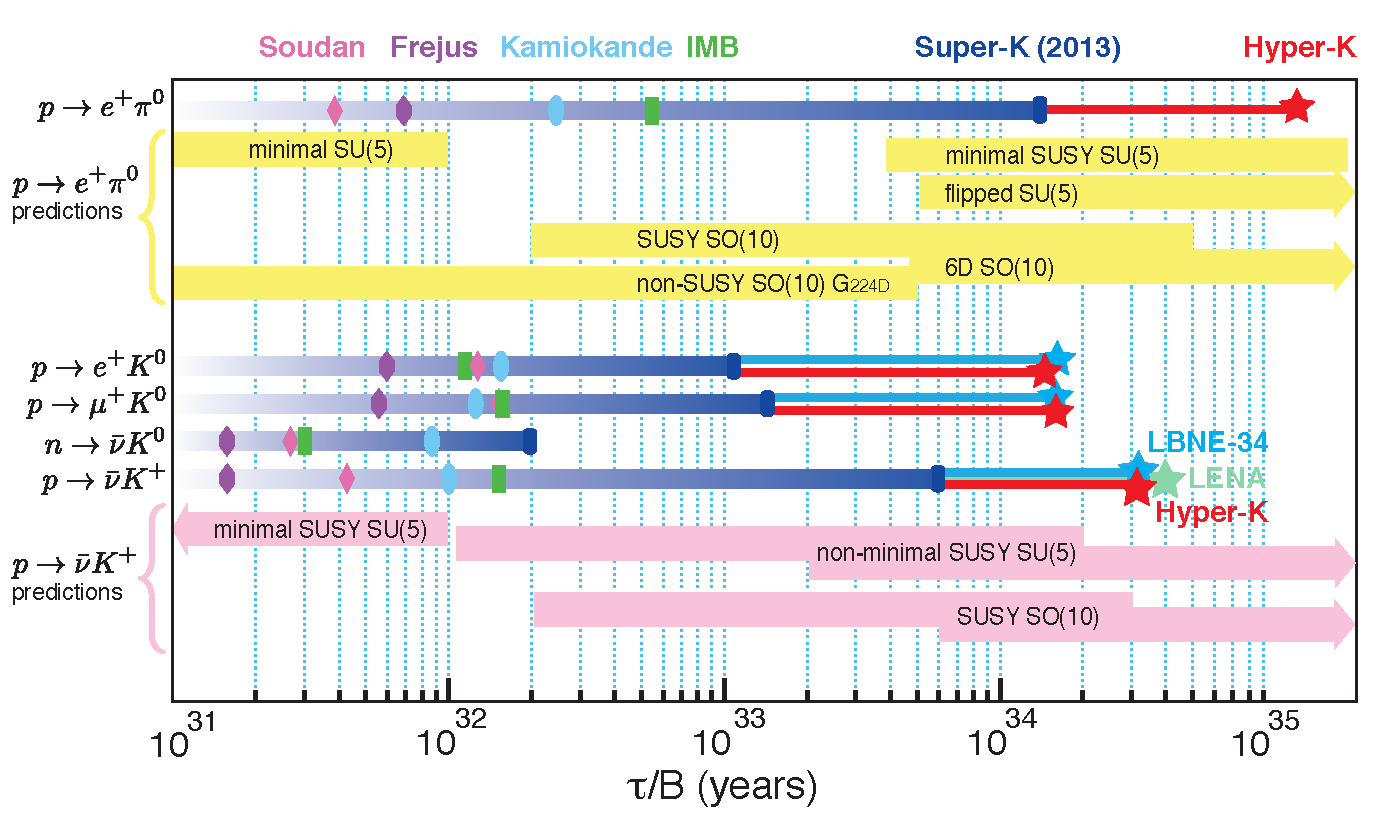
\includegraphics[width=\textwidth]{sklimits_compare_theory_2013_hklenalbne.pdf} <---UPDATED!!
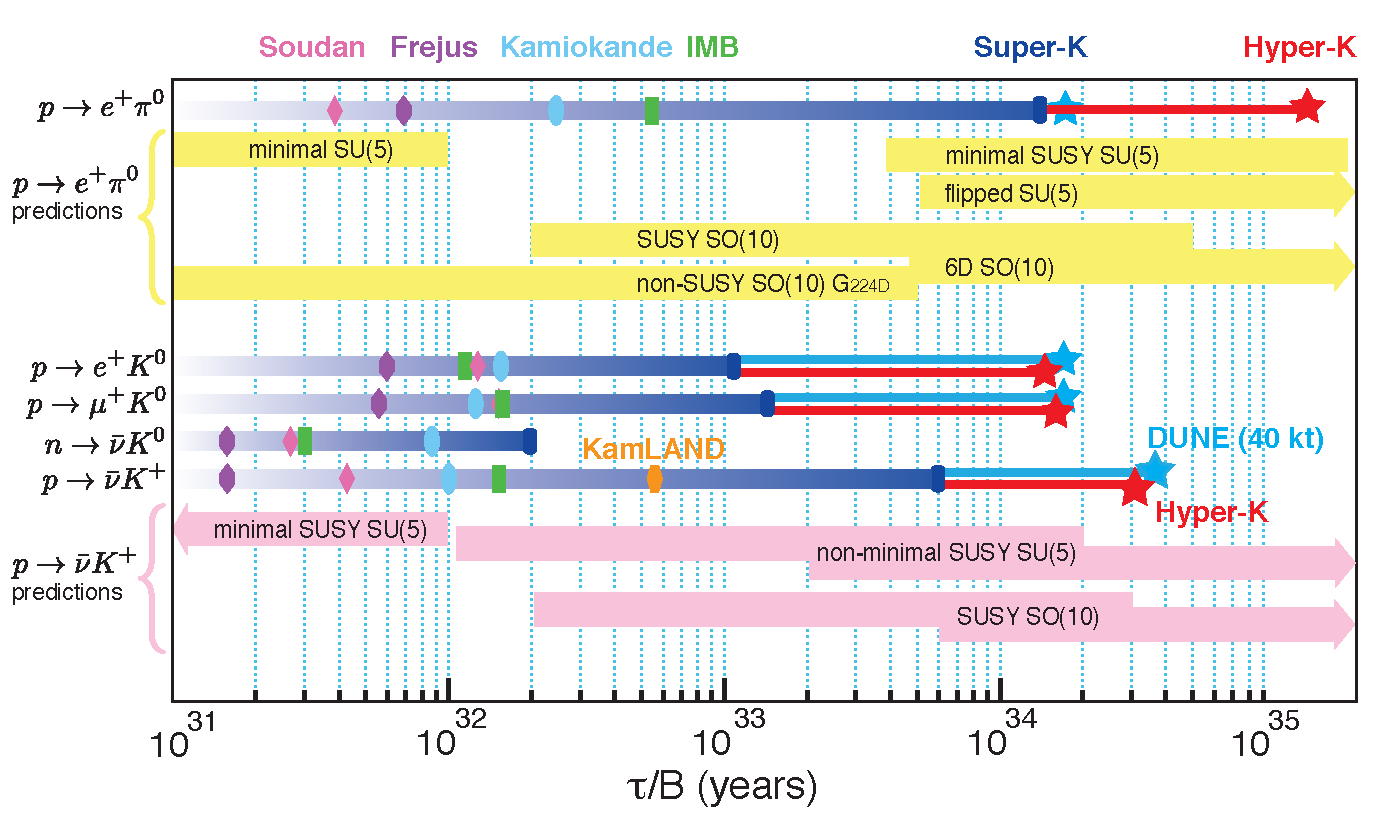
\includegraphics[width=\textwidth]{sklimits_compare_theory_2015_KamLAND}
\end{cdrfigure}
%
From this figure it is clear that an experiment such as DUNE with sensitivity to proton lifetimes
between $10^{33}$ and $10^{35}$ years will probe a large number of GUT models, and 
thus will present a compelling opportunity for discovery.
Even if no proton decay is detected, stringent lifetime limits will constrain 
the models: minimal SU(5) was ruled out by the early work of IMB and
Kamiokande, and minimal SUSY~SU(5) is considered to be ruled out by \superk.
In most cases, another order of magnitude in improved limits will not rule out
specific models but will constrain their allowed parameters;
this could allow identification of less favored models that %must be fine-tuned
would require fine-tuning in order to accommodate the data. %, and that are thus less favored.

It is also clear from Figure~\ref{fig:PDK-limits-theory} that it will not be easy for 
a LArTPC-based detector to make significant inroads on the $p \rightarrow e^+ \pi^0$ 
channel, where background-free high-efficiency searches are possible with large 
water Cherenkov detectors at a lower cost per kt.  For this reason, the 
focus of the remaining discussion is on the channels with kaons, in particular 
$p \rightarrow K^+ \overline{\nu}$.  However, it is important to note that 
the full-scale DUNE far detector would be able to provide confirming evidence 
for $p \rightarrow e^+ \pi^0$ should a signal for this channel start to develop 
in the next-generation water detector at the few-times-$10^{34}$-year level. 

%%%%%%%%%%%%%%%%%%%%%%%%%%%%%%%%%%%%%%%%%%%%%%%%%%%%%%%%%%%%%%%%
%%%%%%%%%%%%%%%%%%%%%%%%%%%%%%%%%%%%%%%%%%%%%%%%%%%%%%%%%%%%%%%%
\subsection{Signatures for Nucleon Decay in DUNE}

Extensive surveys~\cite{Bueno:2007um,Klinger:2015kva} of nucleon decay efficiency 
and background rates for large LArTPCs with various depth/overburden 
conditions provide the starting point for the 
assessment of DUNE's capabilities.  Table~\ref{tab:pdecay} lists selected
modes where LArTPC technology exhibits a significant performance 
advantage (per kt) over the water Cherenkov technology.
This section focuses on the capabilities 
of DUNE for the $p\to K^+\overline{\nu}$ channel, which is seen as the most 
promising from theoretical and experimental 
considerations.  Much of the discussion that follows can be 
applied to the other channels with kaons listed in 
the table.
%
\begin{table}[!htbp]
\caption[Efficiencies and background rates for nucleon decay modes]
        {Efficiencies and background rates (events per \SI{}{\Mtyr}) for nucleon decay 
         channels of interest for a large underground LArTPC~\cite{Bueno:2007um}, and 
         comparison with water Cherenkov detector capabilities.  
         The entries for the water Cherenkov capabilities are based 
         on experience with the \superk{} detector~\cite{kearns_isoups}.  
        }
\begin{center}
\begin{tabular}{$L^c^c^c^c} %$ 
\toprule
\rowtitlestyle
Decay Mode   & \multicolumn{2}{^>{}c}{Water Cherenkov} & 
\multicolumn{2}{^>{}c}{Liquid Argon TPC} \\
\rowtitlestyle
   & Efficiency &   Background & Efficiency &   Background \\ \toprowrule
$p \rightarrow K^+ \overline{\nu}$       & 19\%  &  4   &  97\%   &     1  \\ \colhline
$p \rightarrow K^0 \mu^+$      & 10\%  &  8   &  47\%   &  $<2 $ \\ \colhline
$p \rightarrow K^+ \mu^- \pi^+$ &       &      &  97\%   &     1  \\ \colhline
$n \rightarrow K^+ e^- $        & 10\%  &  3   &  96\%   &  $<2$  \\ \colhline
$n \rightarrow e^+\pi^-$      & 19\%  &  2   &  44\%   &  0.8   \\
\bottomrule
\end{tabular}
\end{center}
\label{tab:pdecay}
\end{table}

The key signature for $p\to K^+\overline{\nu}$ is the presence of an
isolated charged kaon (which would also be monochromatic 
for the case of free protons, with $p=$\SI{340}{\MeV}$/c$).  
Unlike the case of $p\to e^+\pi^0$, where the maximum
detection efficiency is limited to 40--45\% because of inelastic
intranuclear scattering of the $\pi^0$, the kaon in $p\to
K^+\overline{\nu}$ emerges intact (because the kaon momentum is 
below threshold for inelastic reactions)
from the nuclear environment of the decaying proton $\sim 97\%$ of the
time.  Nuclear effects come into play in other ways, however: the kaon
momentum is smeared by the proton's Fermi motion and shifted downward
by re-scattering~\cite{Stefan:2008zi}. 


In LArTPC detectors, the $K^+$ can be tracked, its momentum measured
by range, and its identity positively resolved via detailed analysis
of its energy-loss profile.  This is in sharp contrast with water 
detectors, in which the $K^+$ momentum is below Cherenkov threshold.
Additionally, all decay modes can be cleanly reconstructed 
and identified in an LArTPC, including those with neutrinos,
since the decaying proton is nearly at rest.  With this level of
detail, it is possible for a single event to provide overwhelming
evidence for the appearance of an isolated kaon of the right momentum
originating from a point within the fiducial volume.  The strength of
this signature is clear from cosmogenic-induced kaons observed by the
ICARUS Collaboration in the cosmic-ray (CR) test run of half of the T600
detector, performed at a surface installation in Pavia~\cite{Amerio:2004ze} 
and in high-energy neutrino interactions with the full T600 in the recent 
CNGS (CERN Neutrinos to Gran Sasso) run~\cite{Antonello:2012hu}.
Figure~\ref{fig:icaruskaon} shows a sample event from the CNGS run in
which the kaon is observed as a progressively heavily ionizing track 
that crosses into the active liquid argon volume, stops, and
decays to $\mu\nu$, producing a muon track that also stops and decays
such that the Michel-electron track is also visible. 
%The 3D
%reconstruction of the event is shown in Figure~\ref{fig:icarusk3d}.
%
\begin{figure}[!htb]
\centering
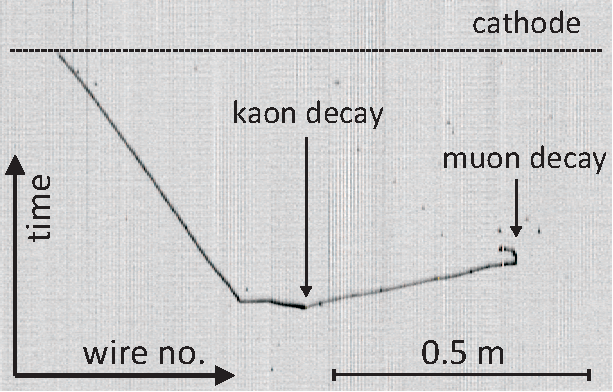
\includegraphics[width=0.72\textwidth]{Fig14a_kaon-coll_raw_R10599E8083.pdf}
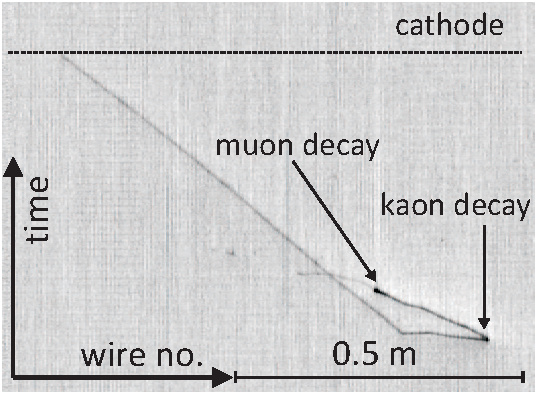
\includegraphics[width=0.72\textwidth]{Fig14b_kaon-ind2_raw_R10599E8083.pdf}
\caption[Decaying kaon observed during the ICARUS run at CNGS]
{Event display for a decaying kaon candidate $K \rightarrow \mu \nu_\mu \ \mu \rightarrow e \nu_e \nu_\mu$ 
in the ICARUS T600 detector observed
in the CNGS data ($K$: \SI{90}{\cm}, \SI{325}{\MeV}; $\mu$ : \SI{54}{\cm}, \SI{147}{\MeV}; 
$e$ : \SI{13}{\cm}, \SI{27}{\MeV}). The top figure shows the signal on the collection plane,
  and the bottom figure shows the signal on the second induction plane~\cite{Antonello:2012hu}.}
\label{fig:icaruskaon}
\end{figure}

References~\cite{Adams:2013qkq,Klinger:2015kva,blake_doc8836} present detailed examinations 
of possible backgrounds, including those arising from cosmic ray interactions in the
detector and surrounding rock, atmospheric neutrino interactions in the
detector, and reconstruction failures. Table~\ref{tab:pdkbkds} summarizes the
results of those background studies.  All together, our estimate of total
background events in the %proton decay 
$p\to K^+\overline{\nu}$ sample is less than 1 \SI{}{\Mtyr}.

%  -(M.Sorel) p.4.67, in Tab.4.2 caption: “background sources and mitigation strategies for the p -> K+ nubar search in DUNE”. right now table may be misunderstood as generic to any proton decay mode. this decay mode should be specified in main text as well, when mention is made to an expected background of less than 1 per Mton*yr (other proton decay modes would have much larger backgrounds)
% AEH added this to lines 311 above and 319 below - as of 12/7/15


\begin{cdrtable}[Background summary for nucleon decay]{lll}{pdkbkds}
{Background sources and mitigation strategies for the $p\to K^+\overline{\nu}$ search in DUNE}
%\begin{center}
%\begin{tabular}{$L^c^c} 
%\toprule
Background Source & Mitigation Strategy  \\ 
\toprowrule
Internal cosmic ray spallation      & Energy threshold \\ \colhline
External cosmogenic & & \\
$K^+$ production  & Depth, fiducialization \\ \colhline
External cosmogenic  & & \\
$K^0$ production & & \\
+internal charge-exchange  & & \\
to $K^+$ & Cuts on other secondaries    \\ \colhline
Atmospheric $\nu$ & & \\ 
$\Delta S=0$ processes & Cut on associated strange baryon \\ \colhline
Atmospheric $\nu$ & Cabibbo-suppressed, & \\ 
$\Delta S=1$ processes &lepton ID \\ \colhline
Atmospheric $\nu$ & $dE/dx$ discrimination, & \\
with $\pi$ mis-ID & 236 MeV muon track \\
\colhline
Reconstruction pathologies & $dE/dx$ profiles vs track length \\
%\end{tabular}
%\end{center}
%\label{tab:pdkbkds}
\end{cdrtable}
%
%%%%%%%%%%%%%%%%%%%%%%%%%%%%%%%%%%%%%%%%%%%%%%%%%%%%%%%%%%%%%%%%%
\subsection{\boldmath Summary of Expected Sensitivity to Key Nucleon Decay Modes}
%\section{\boldmath Expected Sensitivity to $p \rightarrow K^+ \overline{\nu}$}

Based on the expected signal efficiency and upper limits on the
background rates, the expected limit on the proton
lifetime as a function of running time in DUNE for $p \rightarrow K^+
\overline{\nu}$ is shown in Figure~\ref{fig:kdklimit}. 
\begin{figure}[!htb]
\centering
%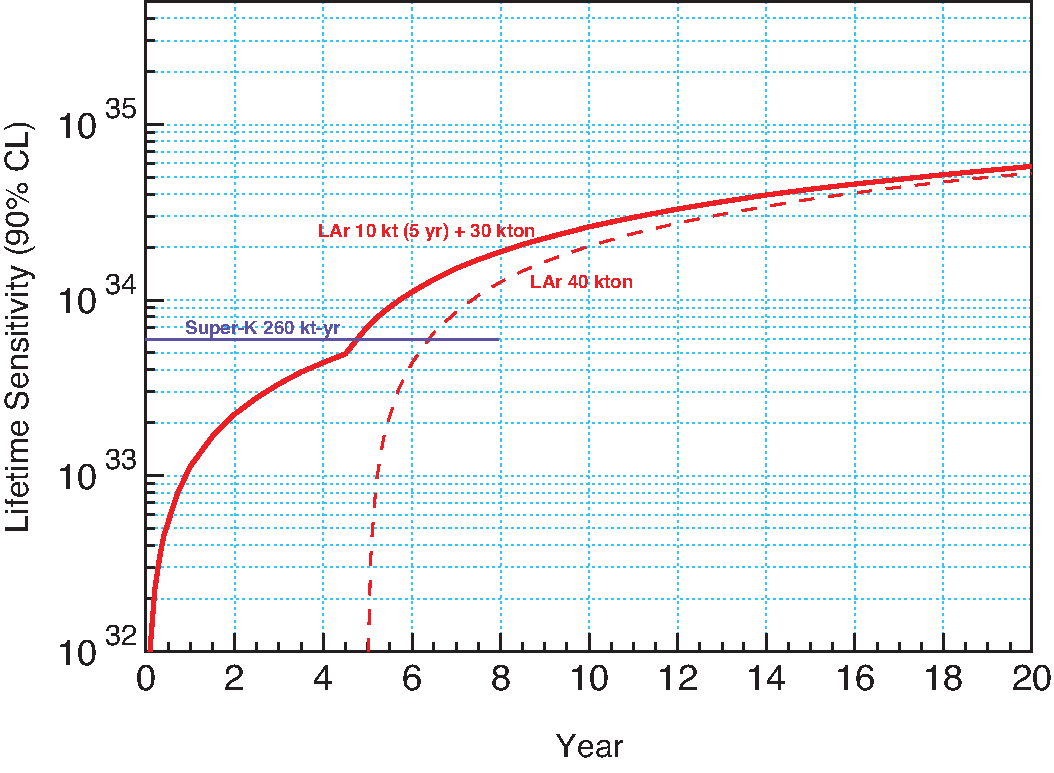
\includegraphics[width=0.8\textwidth]{lar10-40.pdf}
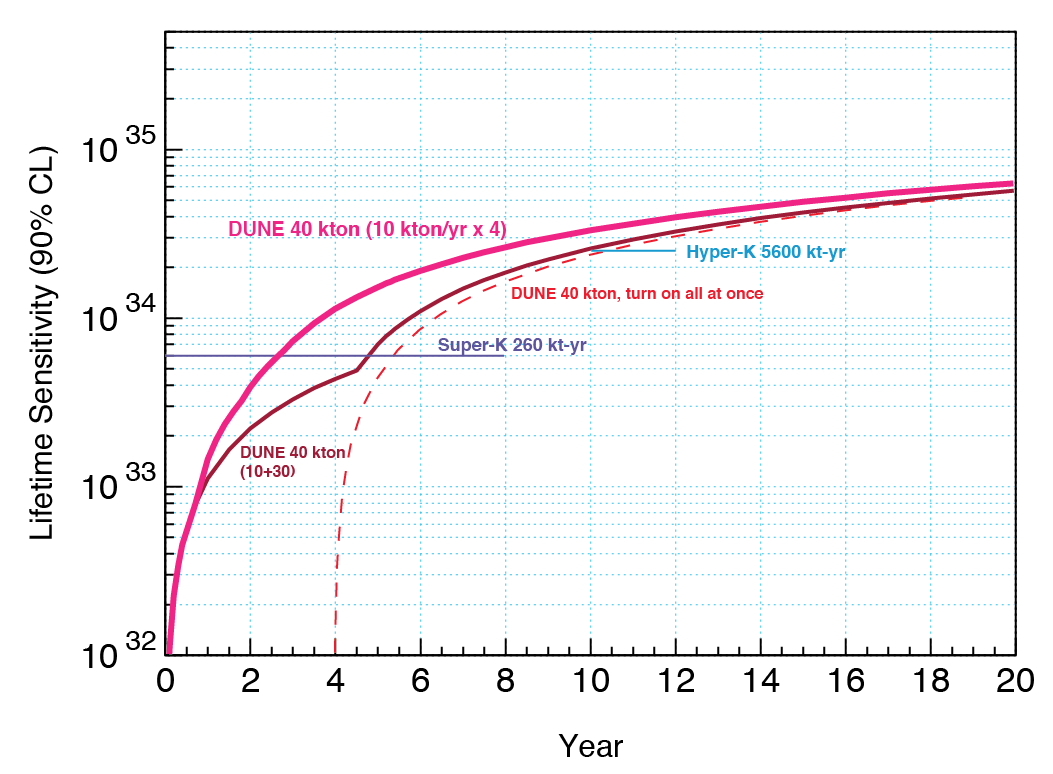
\includegraphics[width=0.8\textwidth]{lar4x10.png}
\caption[Proton decay lifetime limit for $p \rightarrow K^+ \overline{\nu}$
  versus time]{Proton decay lifetime limit for $p
  \rightarrow K^+ \overline{\nu}$ as a function of time for
  underground LArTPCs starting with an initial 10 kt and adding another 10 kt
each year for four years, for a total of 40 kt. 
  For comparison, the current limit from SK and a projected limit from Hyper-K 
is also shown.
  The limits are at 90\% C.L., calculated for
  a Poisson process including background, assuming that the detected events
  equal the expected background.}
\label{fig:kdklimit}
\end{figure}
%

%    REWROTE THIS BELOW     Figure~\ref{fig:kdklimit} 
%This figure demonstrates that 
%to improve the current limits on
%the $p \rightarrow \overline{\nu} K^+$, set by \superk, significantly
%beyond that experiment's sensitivity, 
%a LArTPC
%detector of at least 10~kt, installed deep underground, is needed.
%A \ktadj{40} detector will improve the current limits by an order of
%magnitude after running for two decades.  Clearly a larger detector
%mass would improve the limits even more in that span of time.


The current limits on
the $p \rightarrow \overline{\nu} K^+$ were set by \superk. This figure demonstrates that 
improving these limits significantly
beyond that experiment's sensitivity would require 
a LArTPC
detector of at least \SI{10}{kt}, installed deep underground. %, is needed.
A \ktadj{40} detector will improve the current limits by an order of
magnitude after running for two decades.  Clearly a larger detector
mass would improve the limits even more in that span of time.


\section{Atmospheric Neutrinos}
\label{sec:physics-atmpdk-atmnu}

Atmospheric neutrinos %are 
provide a unique tool to study neutrino oscillations: the 
oscillated flux contains all flavors of neutrinos and antineutrinos, is very sensitive to 
matter effects and to both $\Delta m^2$ values, %\fixme{check} 
and covers a wide range of L/E. In principle, 
all oscillation parameters could be measured, with high complementarity to 
measurements performed with a neutrino beam. %In addition, 
Atmospheric 
neutrinos are of course available all the time, %in particular 
which is particularly important before the beam becomes 
operational. %Atmospheric neutrinos 
They also provide a laboratory in which to search 
for exotic phenomena where the dependence of the flavor-transition and survival 
probabilities on energy and path length can be defined. The DUNE far detector, 
with its large mass and the overburden to protect it from backgrounds, is an 
ideal tool for these studies. The following discussion will focus on the 
measurement of the oscillation parameters in which the role of atmospheric neutrinos is 
most important. 

The sensitivity to oscillation parameters has been evaluated with a 
dedicated simulation, reconstruction and analysis chain. 
\fixme{HG:  We need references here}
The fluxes of each neutrino species were computed at the far detector location, after 
oscillation. Interactions in the LAr medium were simulated with the GENIE event 
generator. Detection thresholds and energy resolutions based on full 
simulations were applied to the outgoing particles, to take into account 
detector effects. Events were classified as Fully Contained (FC) or 
Partially Contained (PC) by placing the vertex at a random position inside the 
detector and tracking the lepton until it reached the edge of the detector. %its edges.  
Partially Contained events 
are those where a final state muon exits the detector.  The number of events expected 
for each flavor and category is summarized in Table~\ref{tab:atmos_rates}.

%
\begin{cdrtable}
[Atmospheric neutrino event rates]{lc}{atmos_rates}{Atmospheric neutrino event rates including oscillations in \SI{350}{\ktyr} with a LArTPC, fully or partially contained in the detector fiducial volume. }
Sample   &  Event Rate \\ \toprowrule
fully contained electron-like sample   &14,053 \\ \colhline
fully contained muon-like sample       &20,853 \\ \colhline
partially contained muon-like sample   & 6,871 \\ 
\end{cdrtable}
%
\begin{sloppypar}
Figure~\ref{fig:lovere} shows the expected L/E distribution for high-resolution, muon-like 
events from a \SI{350}{\ktyr} exposure. The data provide excellent resolution of the 
first two oscillation nodes, even when taking into account the expected statistical uncertainty.
In performing oscillation fits, the data in each flavor/containment category are 
binned in energy and zenith angle. 
\end{sloppypar}

\begin{cdrfigure}[Reconstructed L/E Distribution of `High-Resolution' Atmospheric Neutrinos]{lovere}
{Reconstructed L/E Distribution of `High-Resolution'
$\mu$-like atmospheric neutrino events in a \SI{350}{\ktyr} exposure with and
without oscillations (left), and the ratio of the two (right), with the
shaded band indicating the size of the statistical uncertainty.}
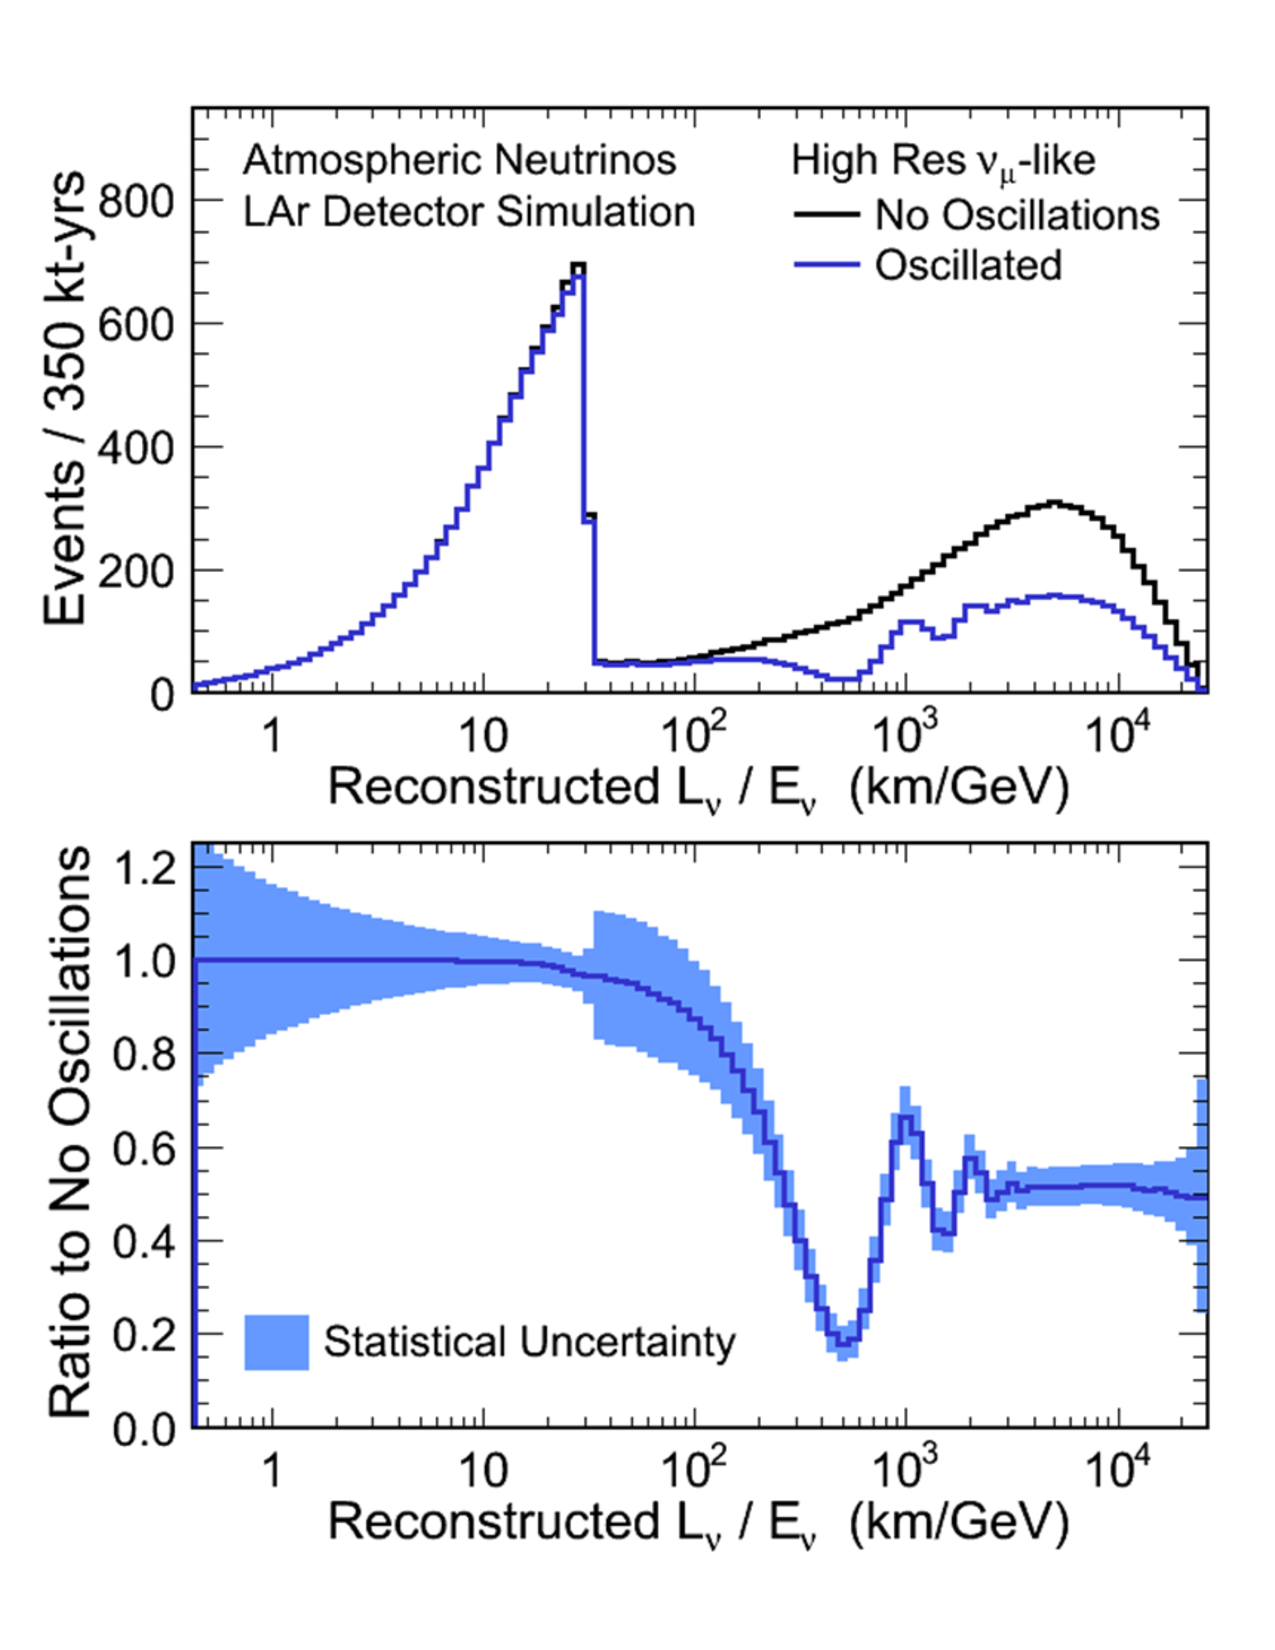
\includegraphics[width=0.45\linewidth]{atm_spectrum_LoverE.pdf}
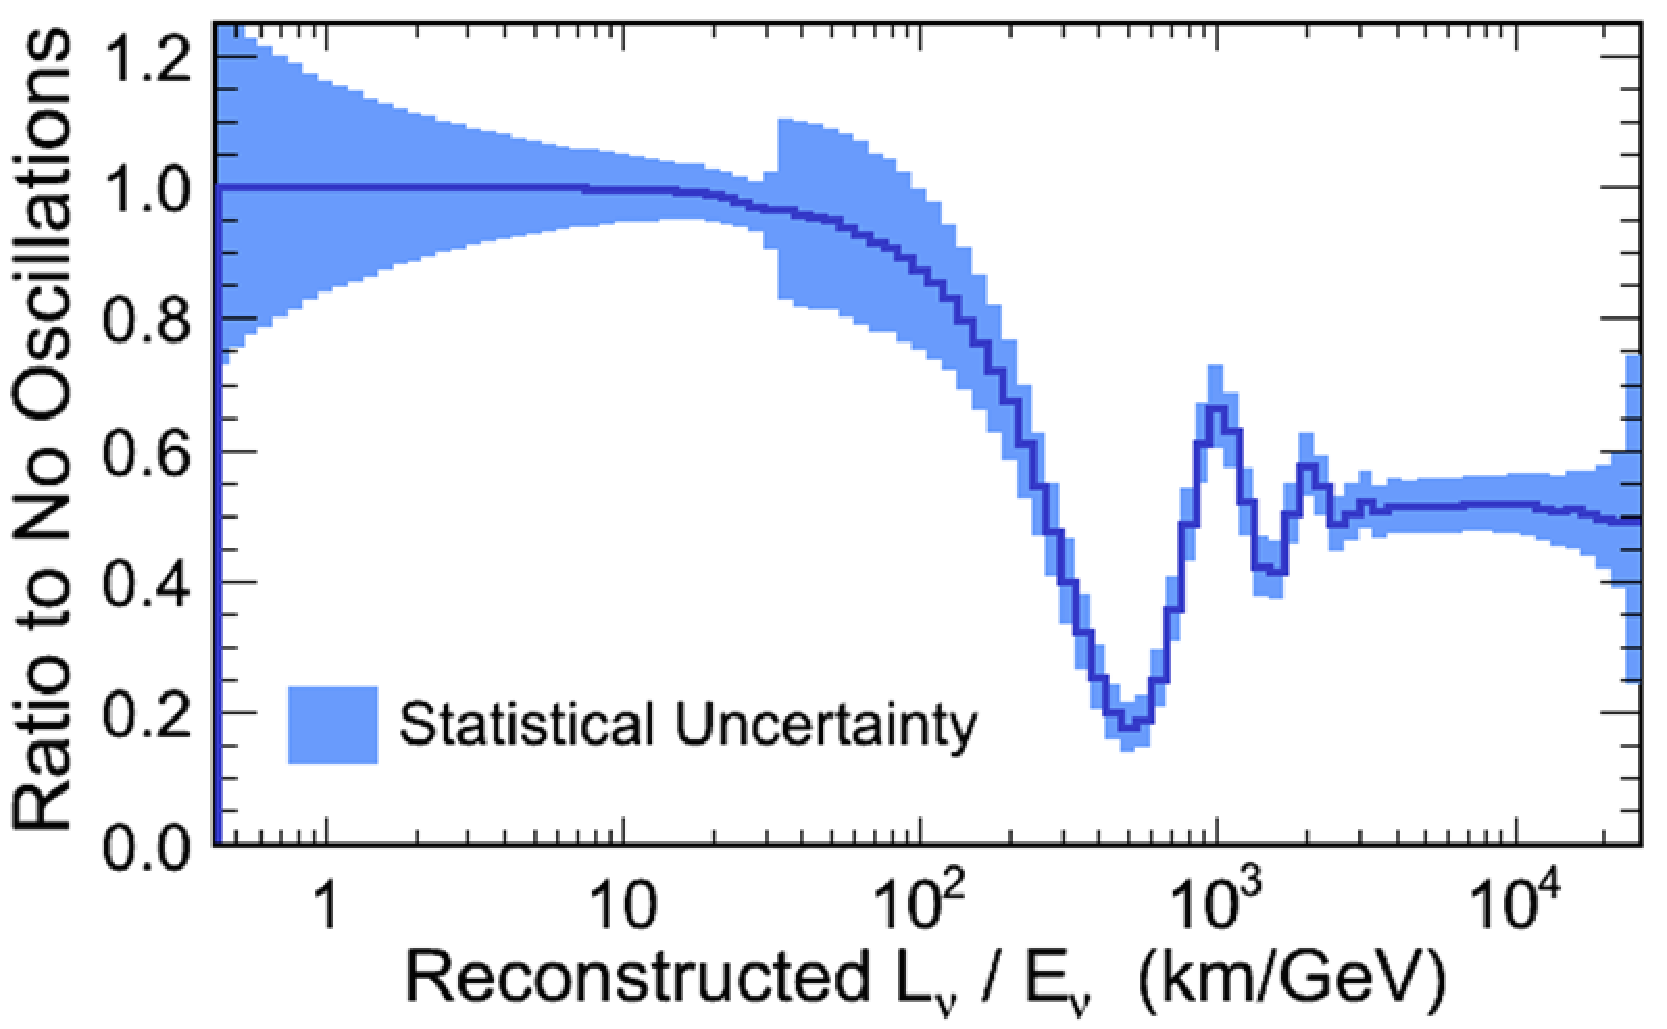
\includegraphics[width=0.45\linewidth]{atm_spectrum_LoverE_2.pdf}
\end{cdrfigure}

When neutrinos travel through the Earth, the MSW resonance influences 
electron neutrinos in the few-GeV energy range. More precisely, the resonance 
occurs for $\nu_e$ in the case of normal mass hierarchy (NH, $\Delta m^2_{32} > 0$), and for 
$\overline{\nu}_e$ in the case of inverted mass hierarchy (IH, $\Delta m^2_{32} < 0$). This is 
illustrated in Figure~\ref{fig:atm_e_zenith}. 

\begin{cdrfigure}[Zenith Angle vs. Energy For Atmospheric Neutrinos]{atm_e_zenith}
{Statistical significance of the difference in expected event rates for NH and IH for 
electron neutrino events (left) and muon neutrino events (right), as a function of neutrino
energy and zenith angle, for a \SI{350}{\ktyr} exposure.}
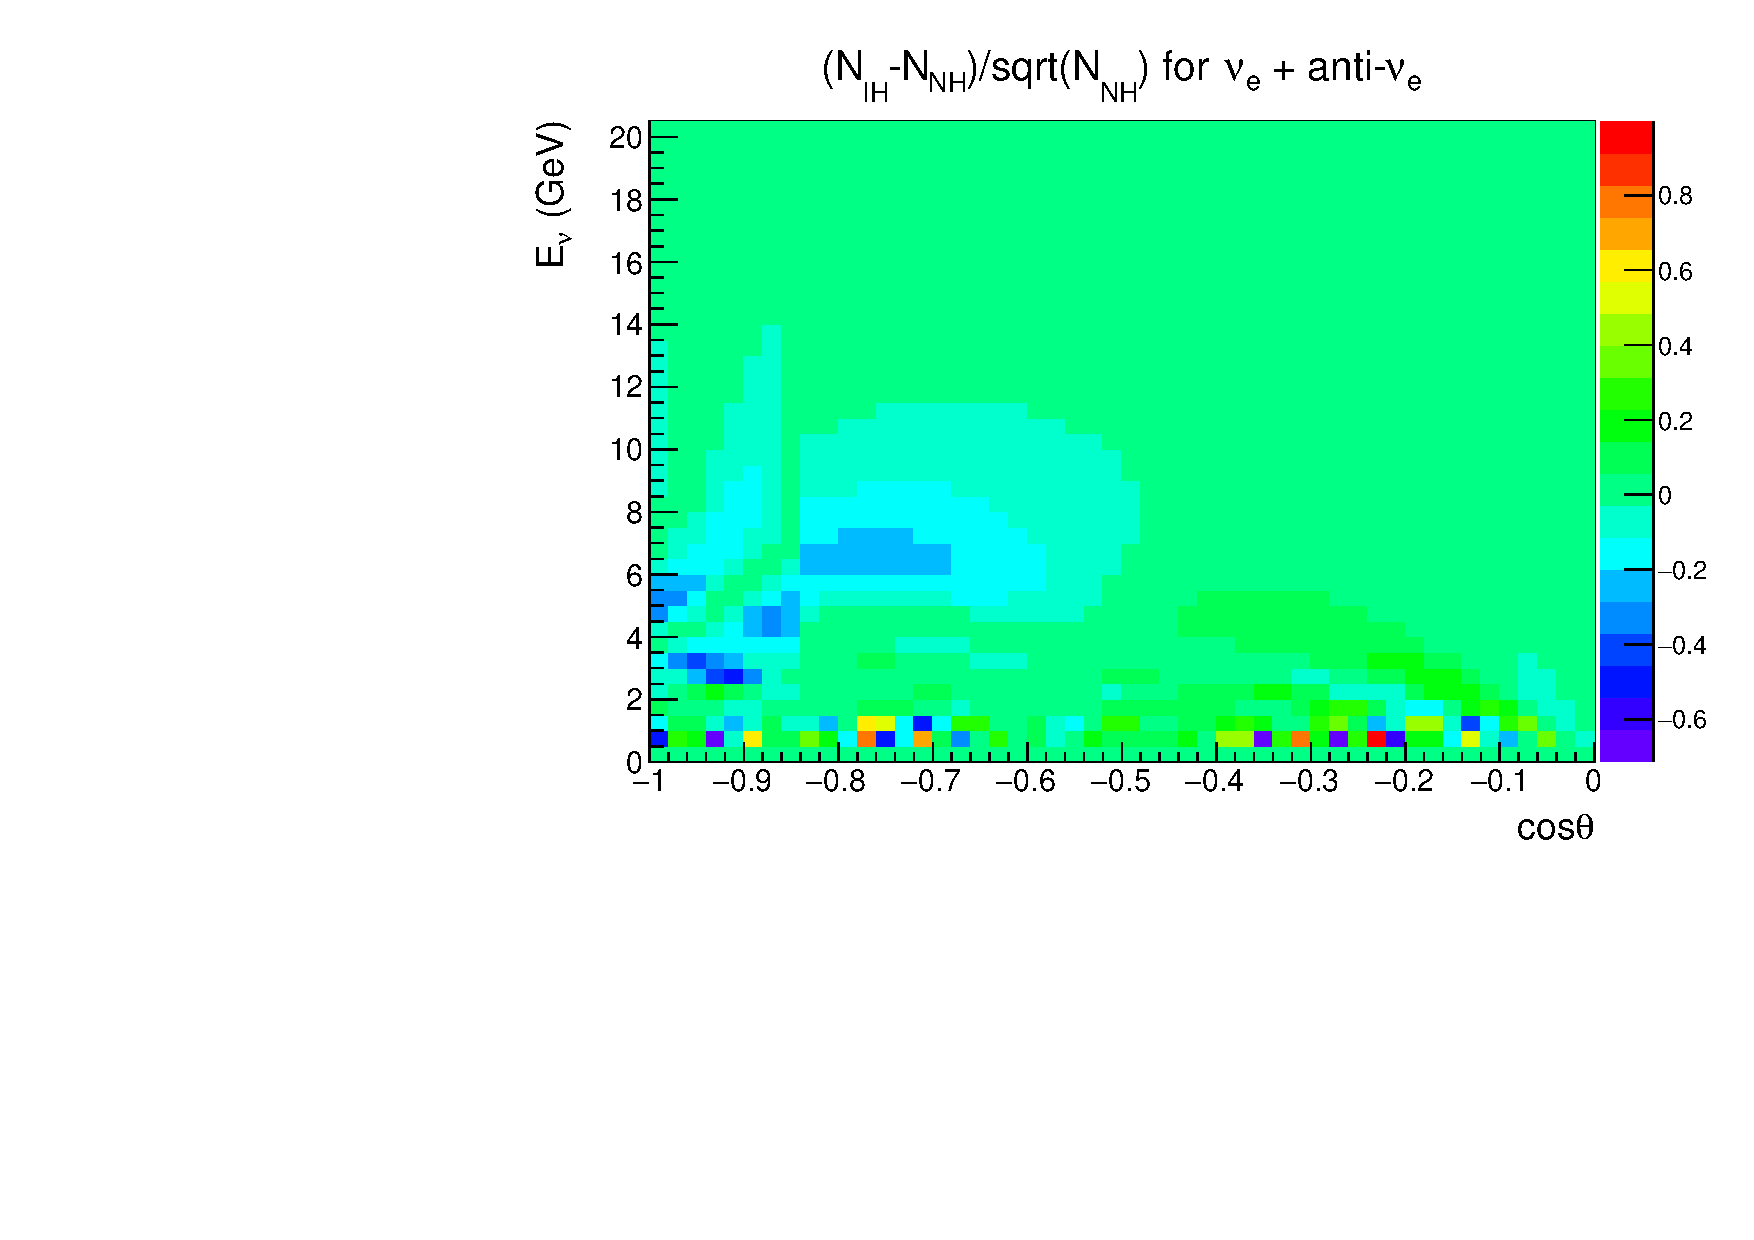
\includegraphics[width=0.45\linewidth]{ElAsym.pdf}
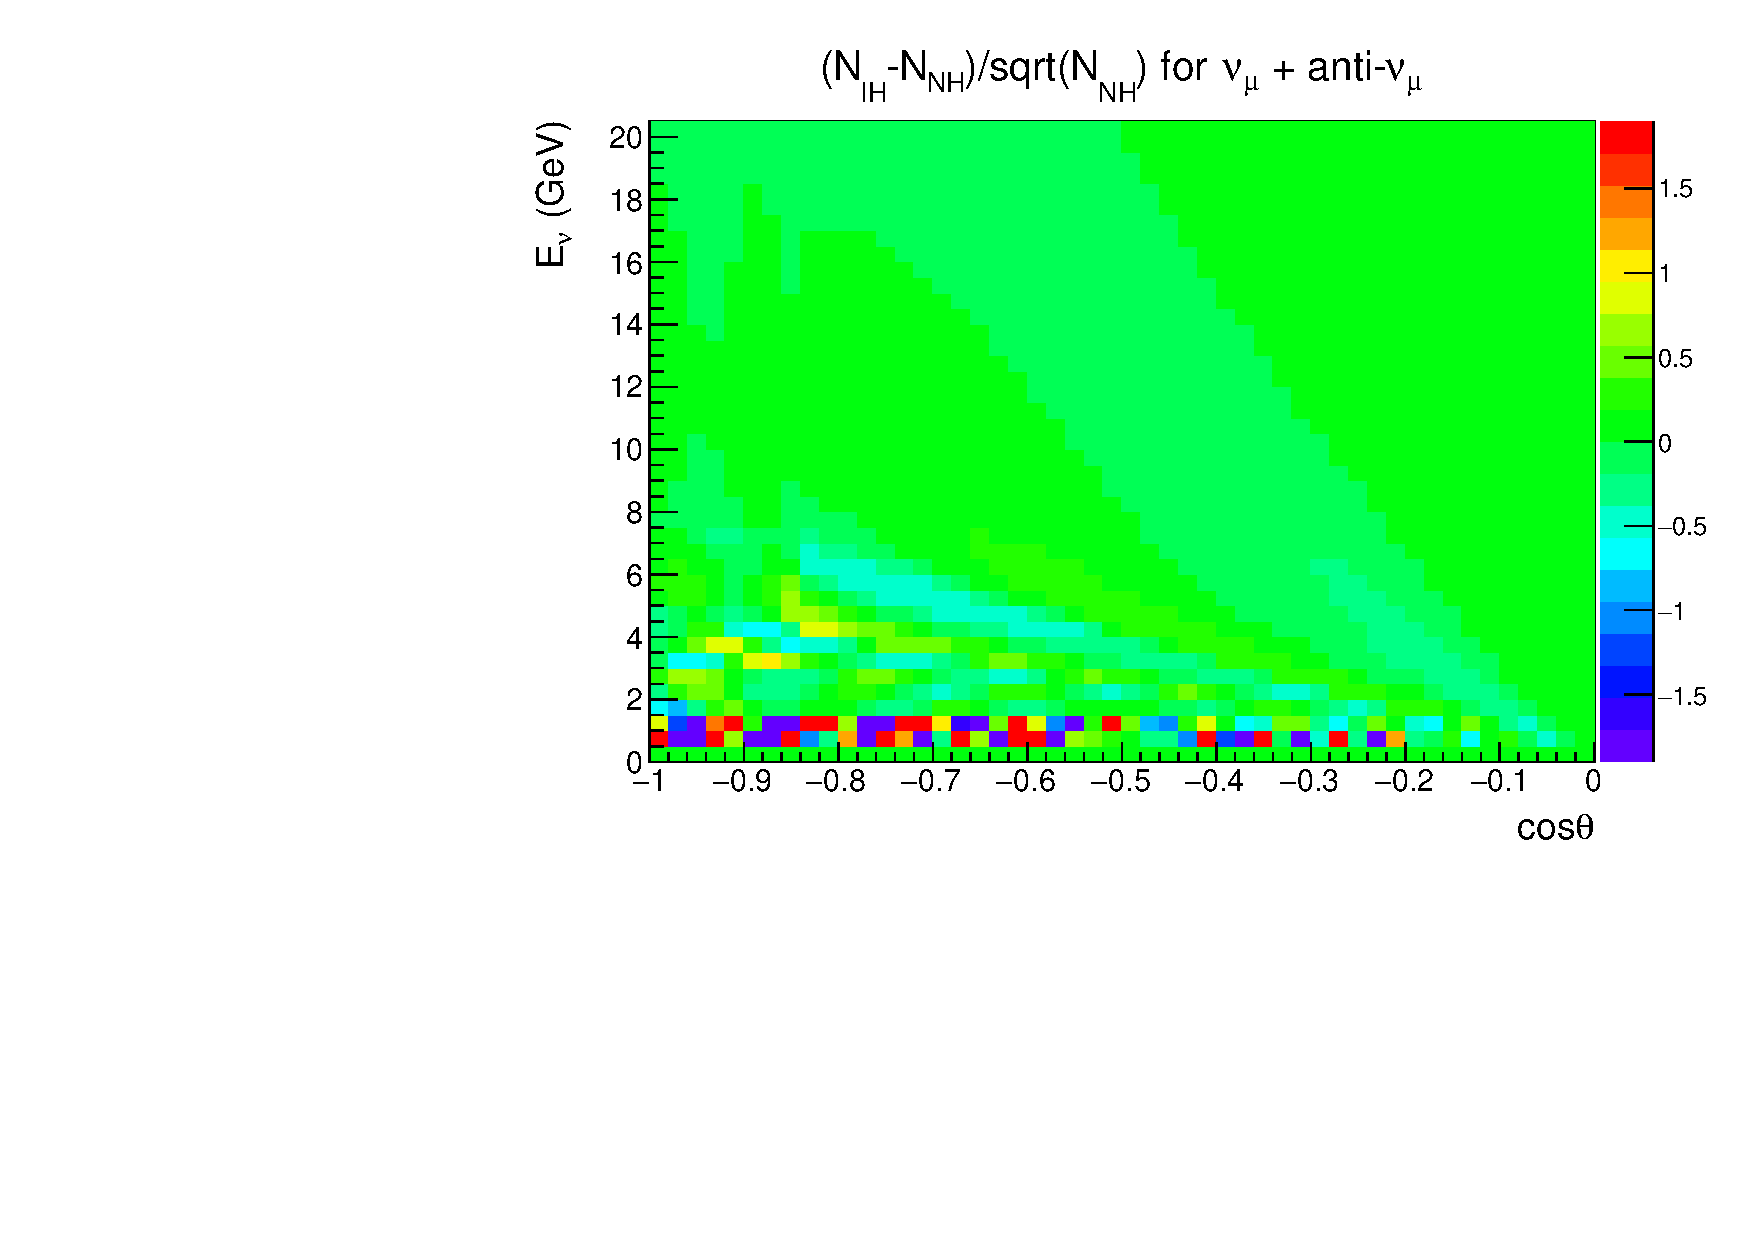
\includegraphics[width=0.45\linewidth]{MuAsym.pdf}
\end{cdrfigure}

The mass hierarchy (MH) sensitivity can be greatly enhanced if neutrino and antineutrino events can be 
separated. The DUNE detector will not be magnetized; however, its high-resolution 
imaging offers possibilities for tagging features of events that provide statistical 
discrimination between neutrinos and antineutrinos. For the sensitivity calculations 
that follow, two such tags were included: a proton tag and a decay electron tag. 
%The 
%reconstructed zenith angle distribution for different event categories is shown in Figure~\ref{fig:atmzenith}.

%\begin{figure}[!htb]
%\centering
%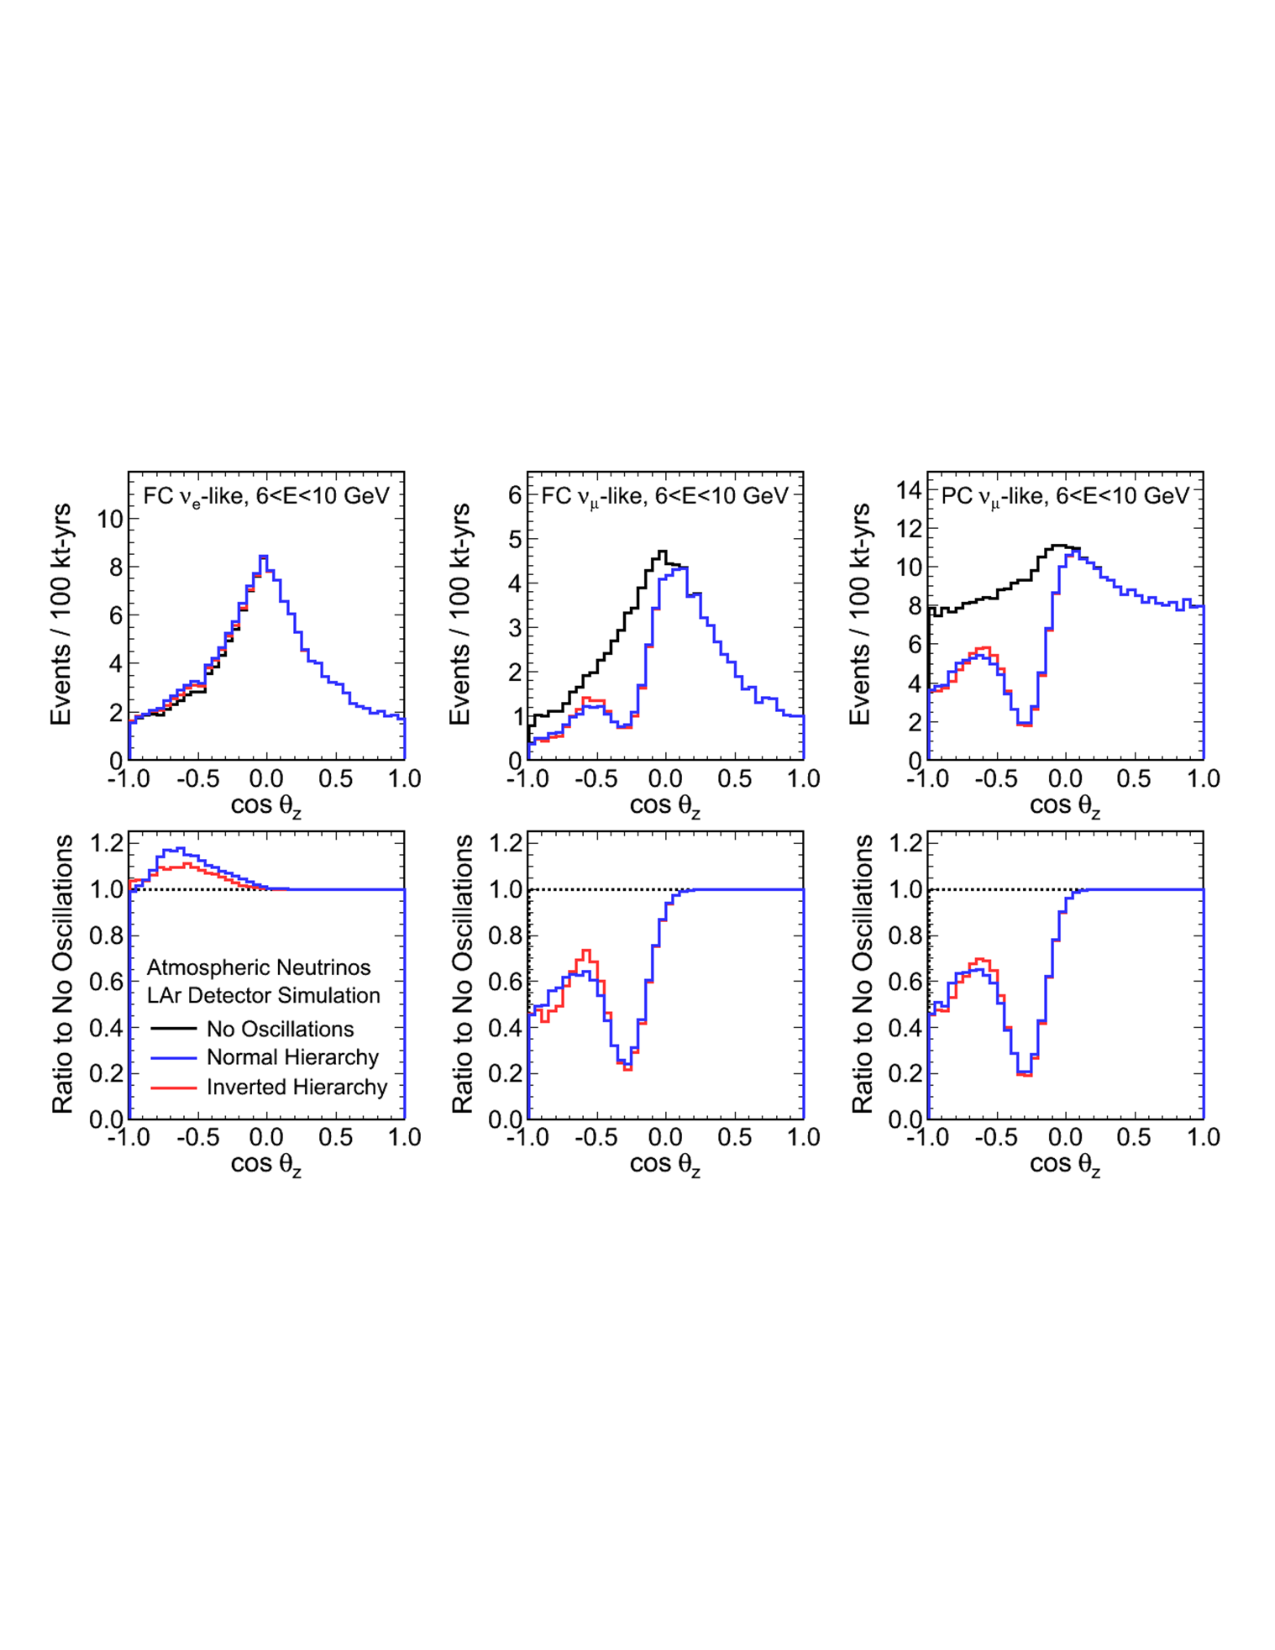
\includegraphics[width=0.95\textwidth]{atm_event_spectra_zenth_6to10gev.pdf}
%\caption[Reconstructed Zenith Angle Distributions for Atmospheric Neutrinos]
%{Reconstructed zenith angle distributions for 6 to 10-GeV events in the different FC and 
%PC samples. Top plots show the expected distributions for no oscillations (black), oscillations with 
%normal (blue), and inverted (red) hierarchy. Bottom plots show the ratio of the normal and inverted 
%expectations to the no-oscillation distributions for each category.}
%\label{fig:atmzenith}
%\end{figure}

Figure~\ref{fig:atm_mh} shows the MH sensitivity as a function of the fiducial exposure. 
Over this range of fiducial exposures, the sensitivity goes essentially as the square 
root of the exposure, indicating that the measurement is not systematics-limited. 
Unlike for beam measurements, the sensitivity to MH with atmospheric neutrinos is 
nearly independent of the CP-violating phase.  The sensitivity comes from both 
electron neutrino appearance as well as muon neutrino disappearance, and is strongly 
dependent on the true value of $\theta_{23}$, as shown in Figure~\ref{fig:atm_mh}.  Despite the
much smaller mass, DUNE would have comparable sensitivity to Hyper-Kamiokande regarding atmospheric 
neutrino analyses~\cite{Kearns:2013lea} due to the higher detector resolution.    

\begin{cdrfigure}[MH Sensitivity vs. Exposure for Atmospheric Neutrinos]{atm_mh}
{Sensitivity to mass hierarchy using atmospheric neutrinos as a function of fiducial 
exposure in a liquid argon detector (left), and as a function of the true value of 
$\theta_{23}$ (right).  For comparison, Hyper-K sensitivities are also shown \cite{Kearns:2013lea}.}  
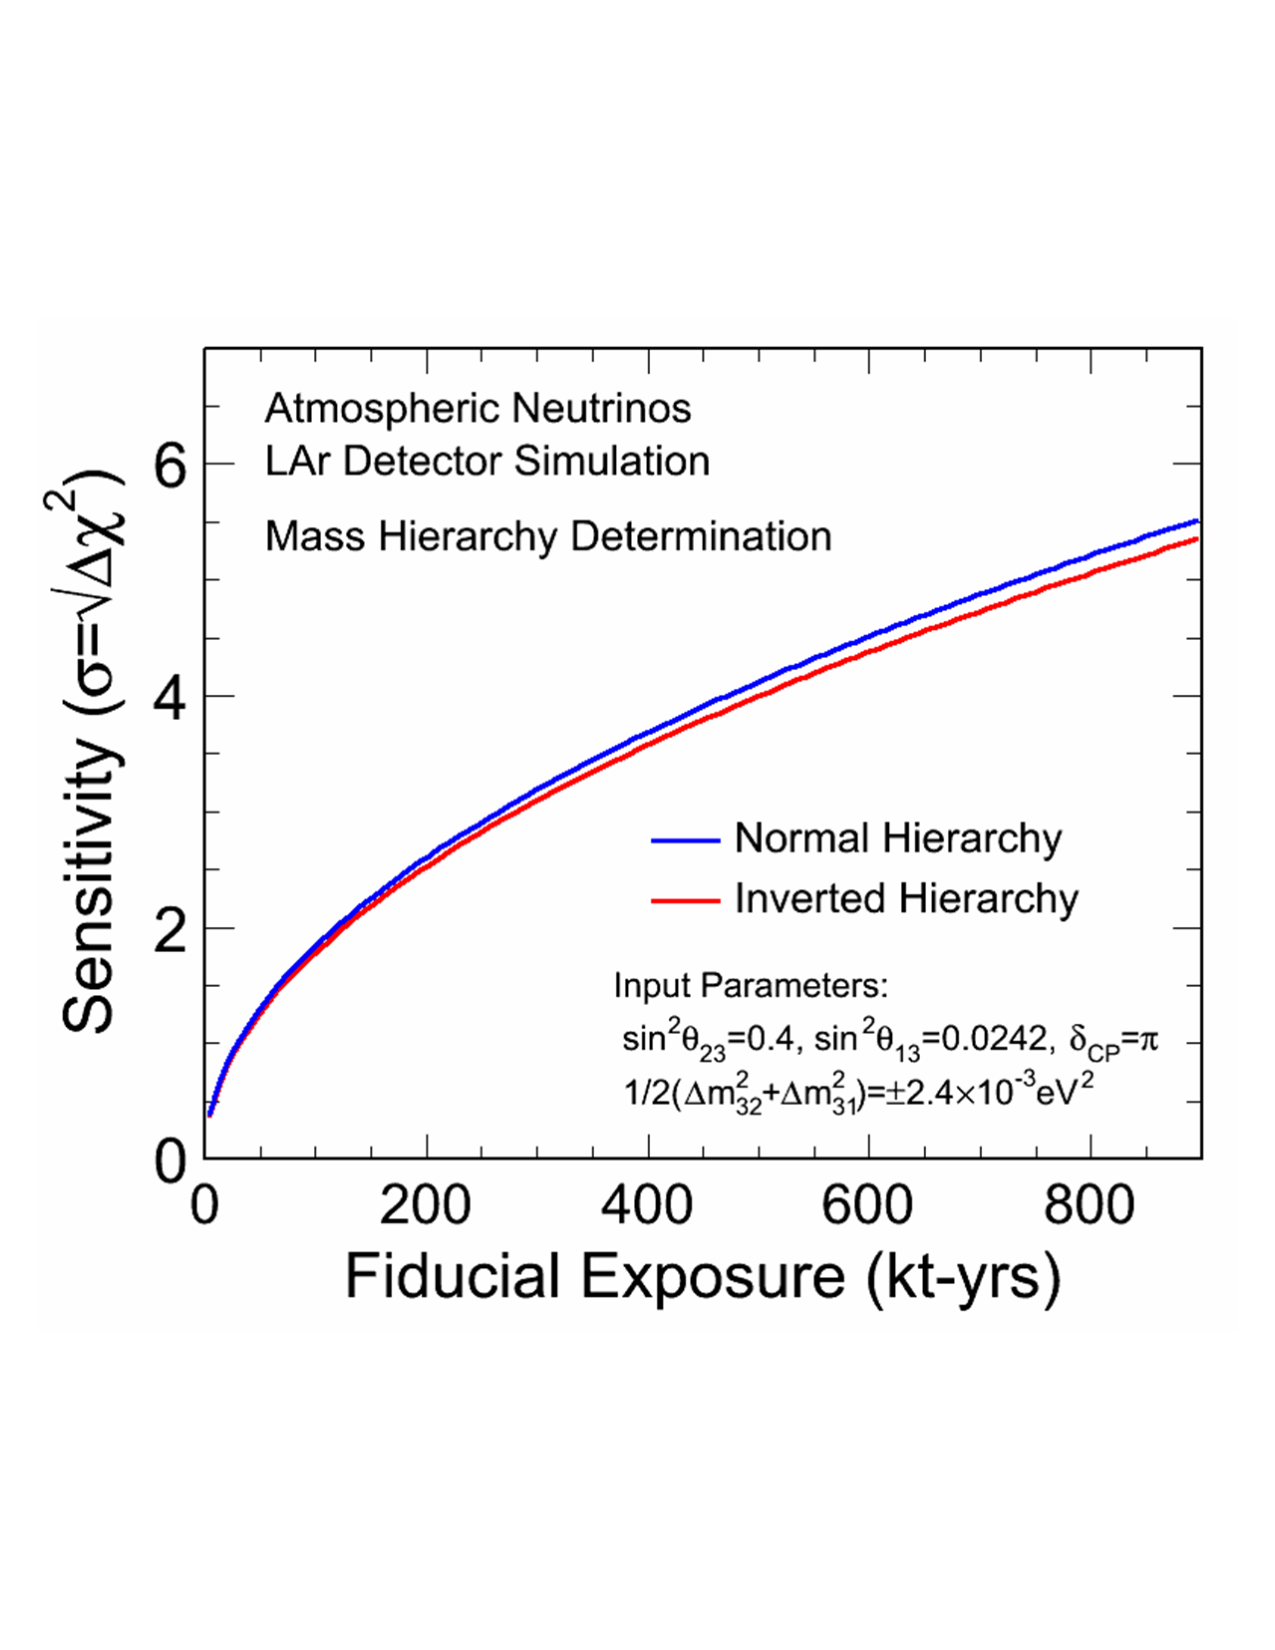
\includegraphics[width=0.42\linewidth]{atm_mh_vs_exposure.pdf}
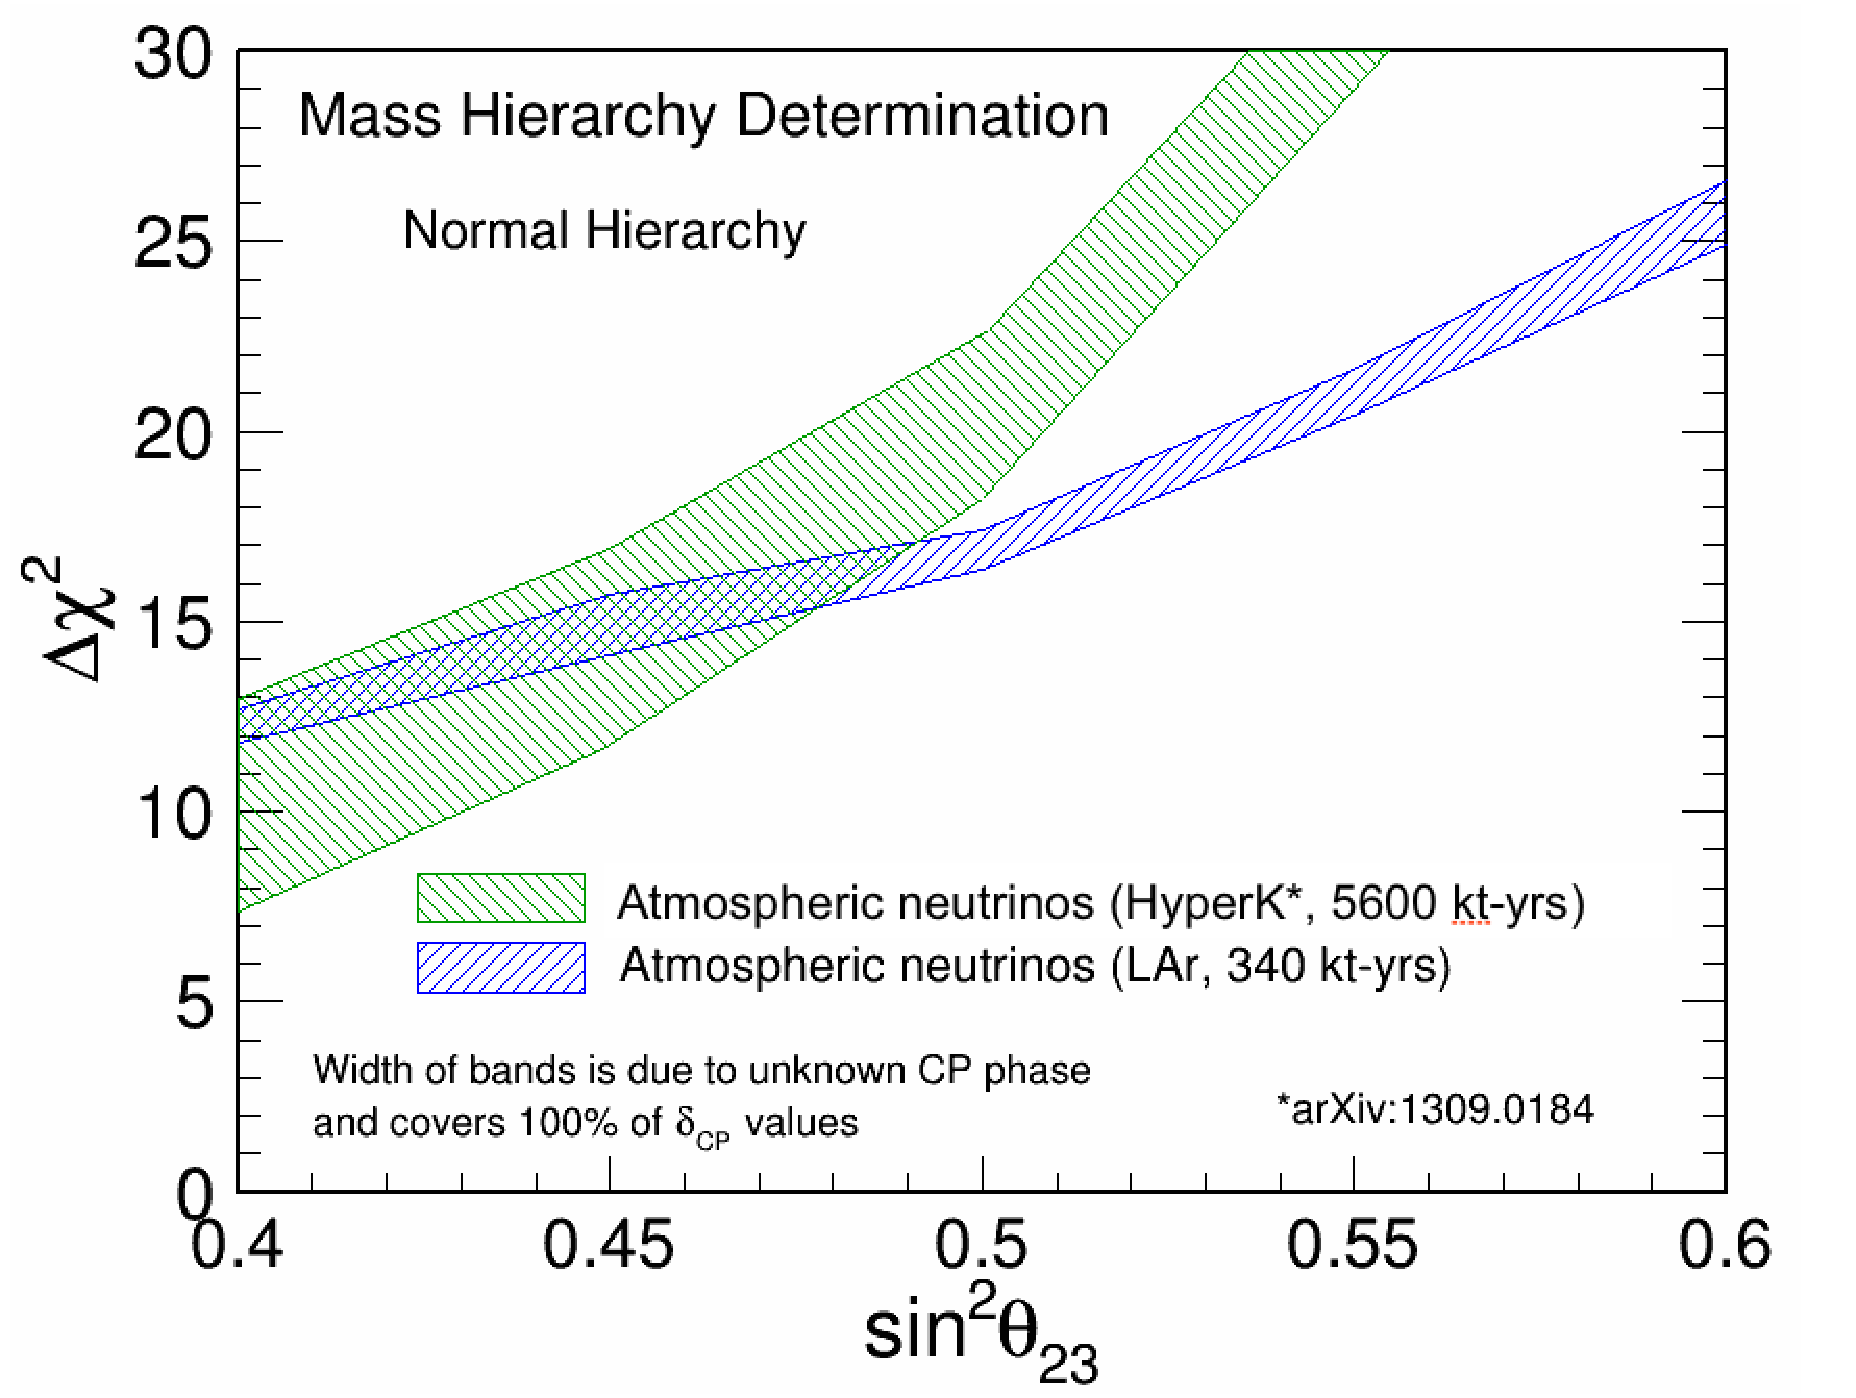
\includegraphics[width=0.48\linewidth]{combined_sensitivity_hierarchy_lbne_vs_hyperk.pdf}
%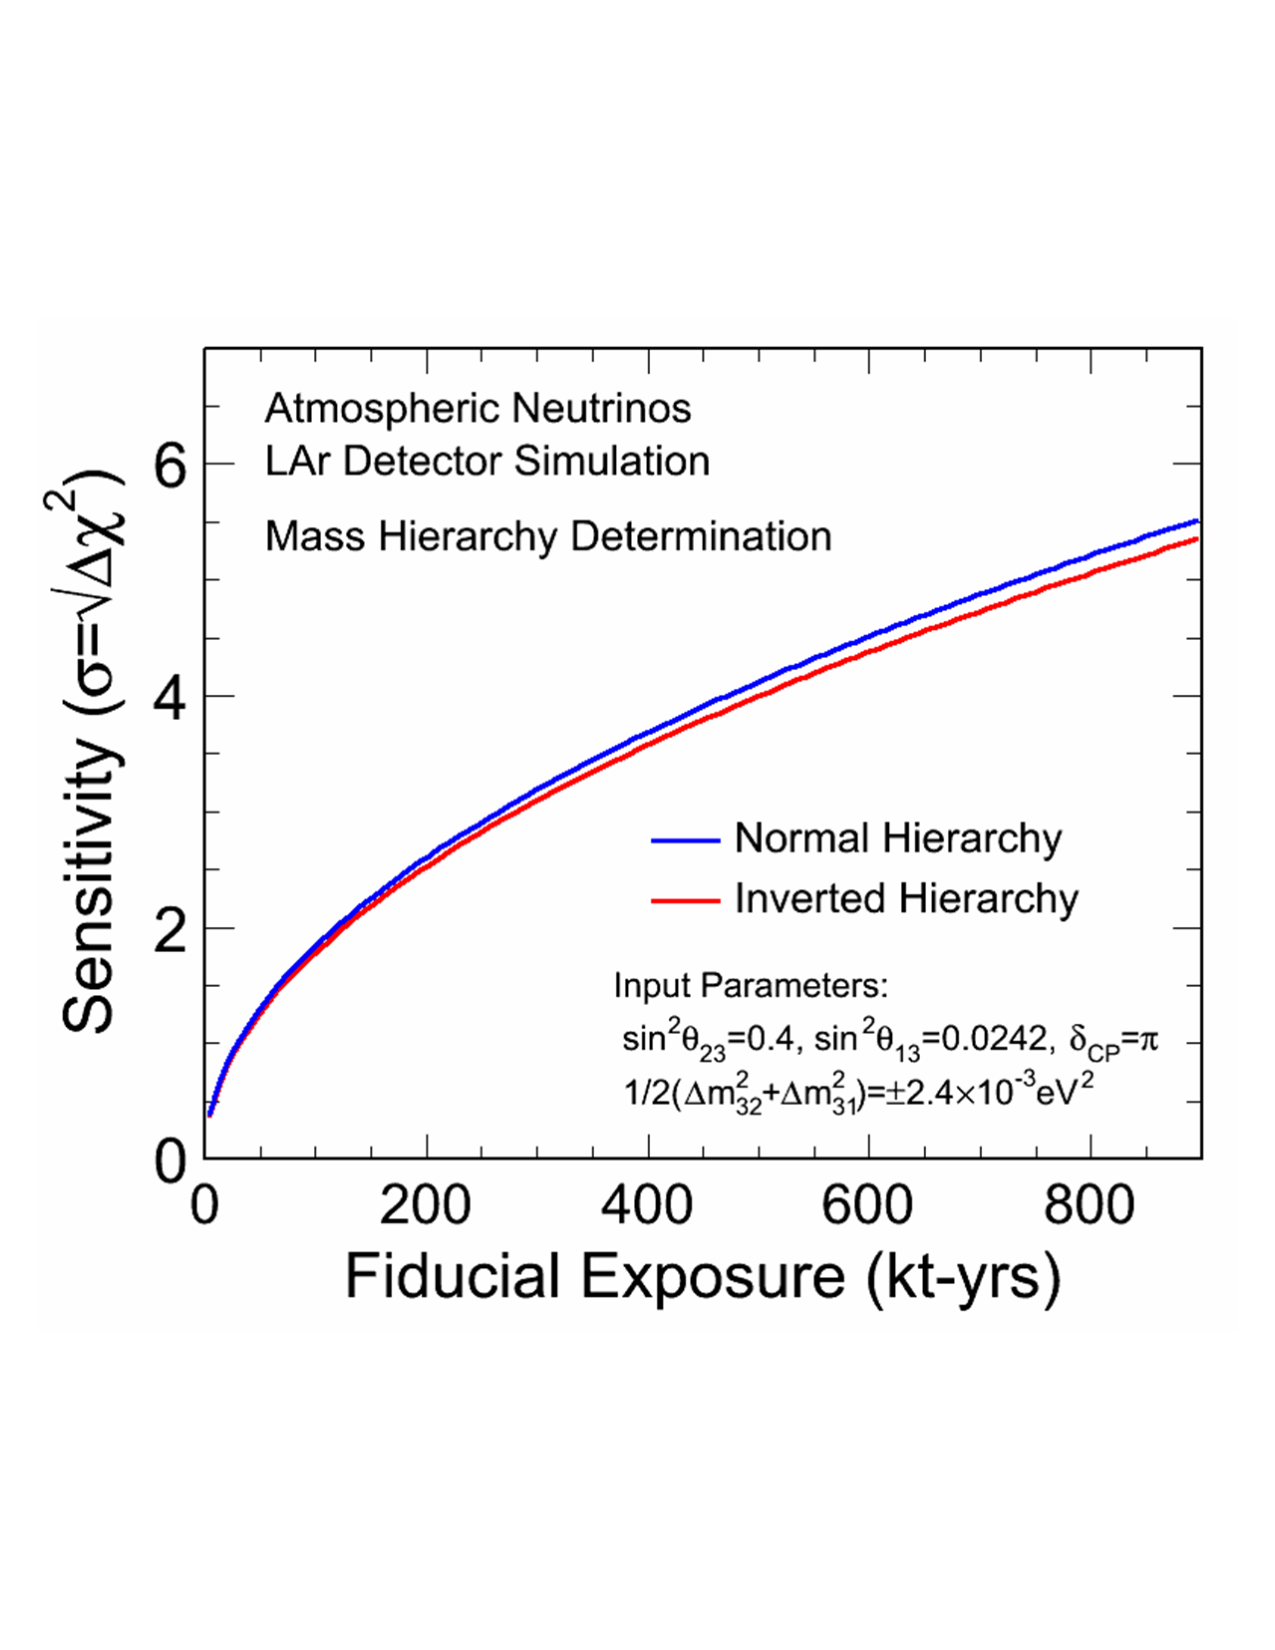
\includegraphics[width=0.50\linewidth]{atm_mh_vs_exposure.pdf}
%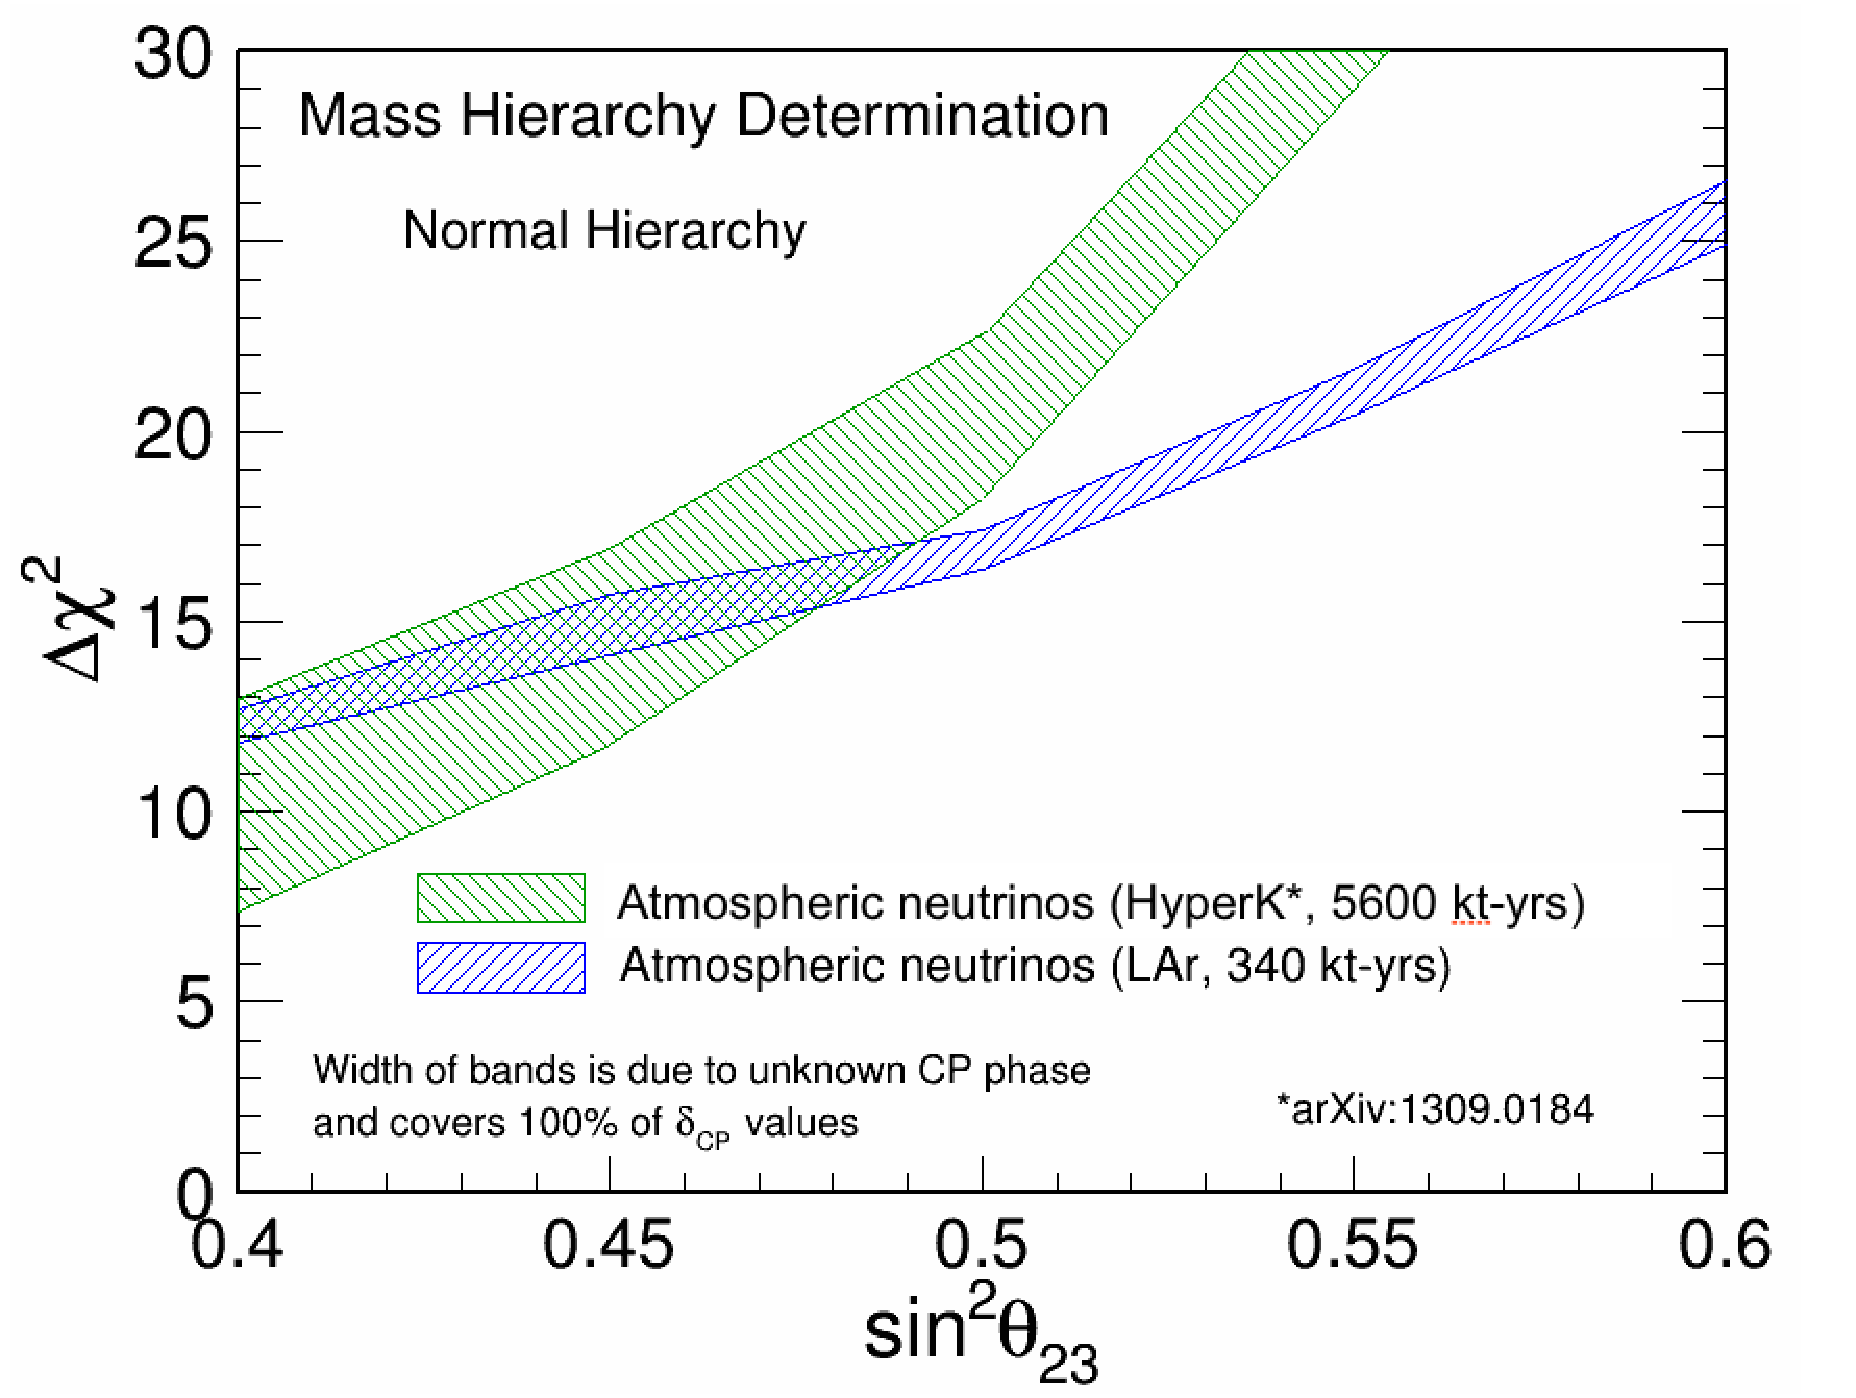
\includegraphics[width=0.50\linewidth]{combined_sensitivity_hierarchy_lbne_vs_hyperk.pdf}
\end{cdrfigure}

In the two-flavor approximation, neutrino oscillation probabilities depend on 
$\sin^2(2\theta)$, which is invariant when changing $\theta$ to $\pi/2-\theta$. In this case, the octant 
degeneracy remains for $\theta_{23}$ in the leading order terms of the full 
three-flavor oscillation probability, making it impossible to determine whether $\theta_{23}< \pi/4$ or 
$\theta_{23}> \pi/4$. Accessing full three-flavor oscillation with atmospheric neutrinos 
will provide a handle for solving the ambiguity.

%The sensitivity to the $\theta_{23}$ octant is shown in Figure~\ref{fig:atm_octant}. 
%With the nominal exposure of \SI{340}{\ktyr}, DUNE will be able to distinguish between 
%octants at 3$\sigma$ significance, based on atmospheric data alone, for true values of [quantify], 
%for any value of $\delta_{CP}$.

%\begin{figure}[!htb]
%\centering
%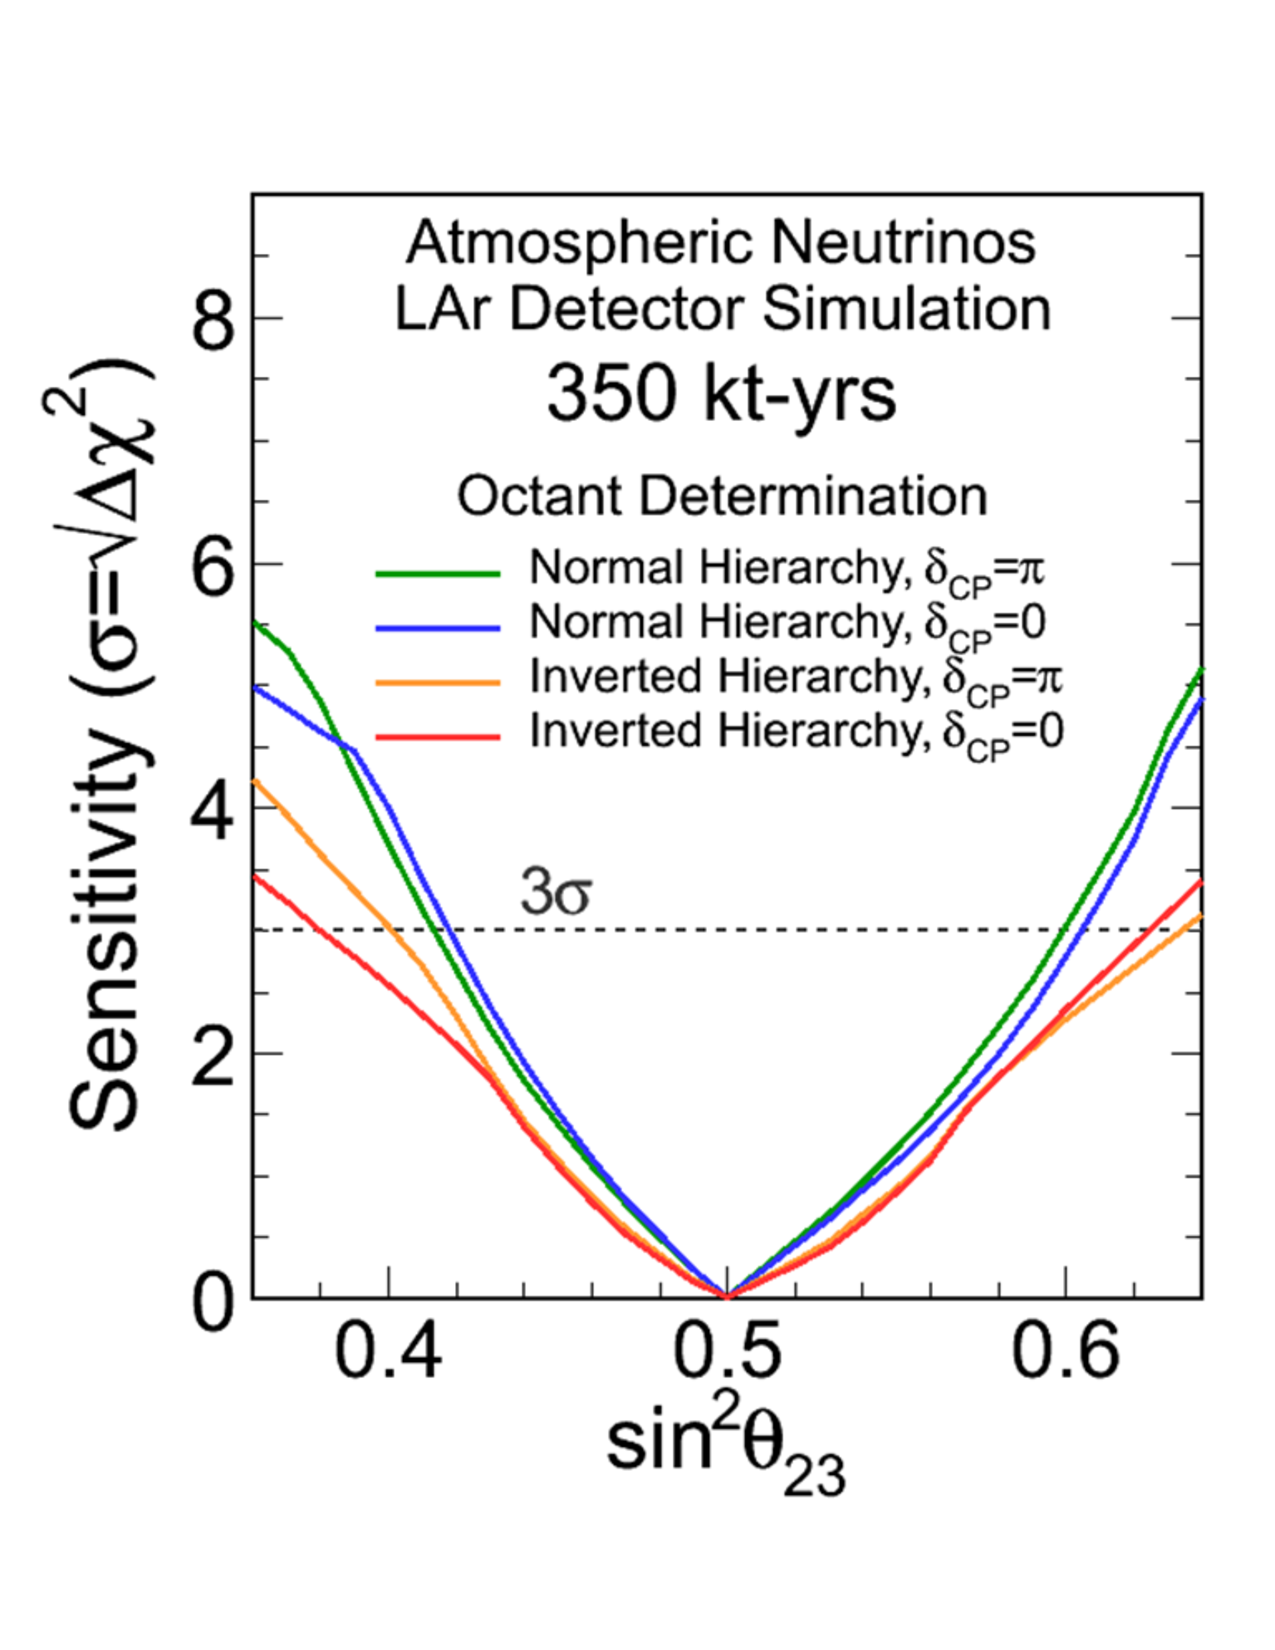
\includegraphics[width=0.60\textwidth]{atm_octant_sens.pdf}
%\caption[Octant Sensitivity for Atmospheric Neutrinos]
%{Sensitivity to $\theta_{23}$ octant for atmospheric neutrinos.}
%\label{fig:atm_octant}
%\end{figure}

%The sensitivity of atmospheric neutrinos to CPV is quite limited and will not reach 
%$3\sigma$ with the nominal exposure, as shown in Fig. 4.27.

These analyses will provide an approach complementary to that of beam neutrinos. 
% Atmospheric neutrinos  can help to lift
For instance, they should enable resolution of 
degeneracies that can be present in beam analyses, since % through the fact that 
the MH sensitivity is essentially independent of $\delta_{CP}$.   Atmospheric neutrino data will be acquired 
even in the absence of the beam, and will provide a useful sample for the development of 
reconstruction software and analysis methodologies.  
Atmospheric neutrinos provide a window into a range of new physics scenarios, and %can 
may allow DUNE to place limits on CPT violation~\cite{Kostelecky:2003cr}, 
non-standard interactions~\cite{Chatterjee:2014gxa}, mass-varying neutrinos~\cite{Abe:2008zza}, 
sterile neutrinos~\cite{Abe:2014gda}, and
Lorentz invariance violation~\cite{Kostelecky:2011gq}.

\section{Indirect Search for WIMPs at the DUNE Far Detector}

If the true nature of DM does indeed involve a weakly interacting particle (WIMP) with a mass in the 100's of GeV range, one of the main search strategies involves looking in astrophysical data for anomalous signals from the %its 
annihilation (or decay) of a WIMP into SM particles, like neutrinos. Signals of DM via neutrinos can come from such distant objects as the galactic center, the center of the Sun or even the Earth~\cite{Press:1985ug,Silk:1985ax,Gaisser:1986ha,Gould:1987ir,Cirelli:2005gh}. As our solar system moves through the DM halo, WIMPs interact with nuclei %of celestial bodies 
 and become trapped in a body's gravitational well.  Over time, the WIMPs accumulate near the core of the body, enhancing the possibility of annihilation. The high-energy neutrinos ($E\sim m_{\rm WIMP}$) from these annihilations can free-stream through the astrophysical body and emerge roughly unaffected (although oscillation and matter effects can slightly alter the energy spectrum).  For the Sun, the background of neutrinos is produced at much lower energies via the nuclear fusion process. Thus, the detection of high-energy neutrinos pointing from the Sun and detected in the DUNE far detector would be clear evidence of DM annihilation.  Since the DUNE far detector has relatively large mass, of the order tens of kt, it can act as a ``neutrino telescope'' and be used to search for signals of DM annihilations coming from the Sun and/or the core of the Earth.  IceCube~\cite{Aartsen:2012kia} and Super-Kamiokande~\cite{Choi:2015ara} have searched for WIMPs with masses from a few to a few hundred GeV$/c^2$ using this method, but have not observed a signal of DM annihilation into neutrinos.  These indirect-detection experiments  are limited by atmospheric neutrino background.  Compared to these experiments, which are based on Cherenkov light detection, the DUNE LArTPC can provide much better angular resolution. This would substantially reduce the background in the direction of the expected WIMP-induced neutrino signal, and could potentially provide competitive limits in the low-WIMP-mass range.  Studies are needed to investigate the sensitivity of DUNE for indirect WIMP detection.
%The mass of the IceCube's $1~km^{3}$ ice volume is of the order $\sim2.6 \times 10^{4}$ times that of the 34-kt DUNE far detector. This requires the DUNE far detector to perform $\sim2.6 \times 10^{4}$ better than IceCube. While this factor seems quite daunting, if not out right impossible, more thorough studies are needed to investigate possible improvements in various performance factors to accomplish this level of enhancement.

\section{Detector Requirements}
\label{sec:physics-atmpdk-detector-requirements}

Physics with atmospheric neutrino interactions and searches for
nucleon decays have several requirements that are not necessarily in
common with the beam-related physics program.  Detector mass and depth plays a
more critical role here; the atmospheric ``beam'' is fixed, and the
number of nucleons available to decay obviously depends on the number
of nuclei in the detector.  The DUNE Far Detector
Requirements~\cite{lbnfdune-cdr-req} specific to searches for proton
decay and measurements of the atmospheric neutrino flux are as
follows:

\begin{itemize}

\item Far Detector Depth: The far detector shall be located at
  sufficient depth to allow detection of atmospheric neutrinos and
  proton decay with negligible backgrounds from cosmogenic sources.
  Depth plays a greater role for these physics topics than for
  long-baseline neutrino oscillations, because of the lack of a beam
  gate coincidence. As discussed in the previous sections, cosmic ray
  interactions in the surrounding rock and detector dead regions
  can lead to critical backgrounds, or create difficulties for
  reconstruction algorithms. Analyses of
  backgrounds~\cite{Bueno:2007um, Klinger:2015kva, Adams:2013qkq} has
  shown that a depth of 4850 ft is sufficient to reduce these
  backgrounds to negligible levels.

% - p.4-72: statement that Fig.4.4 shows that 10-kt DUNE detector can exceed SK limit on p -> K+ nubar in two years is incorrect. From the figure, the necessary exposure is more like 50 kt*yr
% Maury says: change "two years" to "five years". Done AEH 12/7/15

\item Far Detector Mass: The far-detector fiducial size multiplied by
  the duration of operation [expressed in kiloton-years] shall be
  sufficient to yield a scientifically competitive result on proton
  decay. As Figure~\ref{fig:kdklimit} shows, a \ktadj{10} detector can
  exceed the existing Super-Kamiokande limits for the $p\rightarrow
  K^+ + \bar{\nu}$ nucleon decay channel in five years, and the full \ktadj{40} 
  scope in a much shorter time than that.  For atmospheric neutrinos, a
  detector mass of 40 kt will achieve a mass hierarchy determination
  of better than 3$\sigma$ in 10 years.

%\item Far Detector DAQ: The far detector DAQ must enable data be
%  recorded continuously, outside of any beam gate, and enough
 % information from the front end (including photon system) must be retained
 % through the DAQ chain to allow a trigger on events of interest. Any
 % information that would allow the identification of putative events
%  must be kept, and its efficiency should be higher than the
%  efficiency of all other cuts placed on the data.  The trigger system
%  itself must be able to provide information that allows linking of
%  tracks in different modules of the far detector.

\item Far Detector DAQ: The far detector DAQ must enable continuous recording 
of data, outside of any beam gate, and retain enough
  information from the front end (including photon system) 
  through the DAQ chain to enable a trigger on events of interest. The DAQ must keep any
  information that would allow the identification of putative events, 
 % must be kept, 
  and its livetime fraction should be higher than the
  efficiency of all other cuts placed on the data.  The trigger system
  itself must be able to provide information that allows linking of
  tracks in different modules of the far detector.


\item Far Detector Particle ID: It is required that the separation
  of $K^+$'s and $\pi^+$'s in the Far Detector be sufficient to ensure that
  %good enough to leak
  much less than one event leak into the %proton decay (per M.Sorel, changed 12/7/15)
  $p\to K^+\overline{\nu}$ sample.  Unlike the
  long-baseline physics, proton decay physics requires a rare-process search;
  therefore small tails from e.g., atmospheric neutrino
  interactions creating $\pi^+$s that are mis-identified could be very
  damaging.

\item Far Detector Energy Resolution: It is required that the energy
  resolution be known well enough that its uncertainty is a negligible
  contribution to the measurement of the atmospheric neutrino energy
  spectrum of all flavors and that this uncertainty have a negligible impact on
  background predictions for proton decay.

\end{itemize}

